% Main file: pdfLaTeX. Cover image is included in figures/. No shell escape.
\documentclass[12pt,a4paper]{article}
\usepackage[T2A]{fontenc}
\usepackage[utf8]{inputenc}
\usepackage[english,russian]{babel}
\usepackage{tempora}
\usepackage[left=30mm,right=15mm,top=20mm,bottom=20mm]{geometry}
\usepackage{setspace,indentfirst}
\usepackage{amsmath,amssymb}
\usepackage{graphicx,tikz,float,etoolbox}
\usetikzlibrary{arrows.meta,positioning,calc}
\usepackage{array,tabularx,longtable,booktabs}
\usepackage{enumitem,titlesec,tocloft,needspace}
\usepackage{xcolor,listings}
\usepackage[most]{tcolorbox}
\usepackage{lastpage,xurl}
\usepackage[hidelinks,unicode]{hyperref}
\definecolor{ink}{HTML}{193A59}
\definecolor{accent}{HTML}{157B86}
\definecolor{light}{HTML}{F2F6F8}
\onehalfspacing
\frenchspacing
\setlength{\parindent}{1.25cm}
\setlength{\emergencystretch}{2em}
\clubpenalty=10000
\widowpenalty=10000
\brokenpenalty=10000
\setlist{nosep,topsep=0.45em}
\setlist[enumerate]{leftmargin=*,label=\arabic*.}
\setlist[itemize]{leftmargin=*}
\titleformat{\section}{\Large\bfseries\color{ink}}{\thesection.}{0.6em}{}
\titleformat{\subsection}{\large\bfseries\color{ink}}{\thesubsection.}{0.6em}{}
\titleformat{\subsubsection}{\normalsize\bfseries}{\thesubsubsection.}{0.6em}{}
\titlespacing*{\section}{0pt}{2ex}{1.1ex}
\titlespacing*{\subsection}{0pt}{2ex}{1ex}
\setcounter{tocdepth}{2}
\renewcommand{\cftsecleader}{\cftdotfill{\cftdotsep}}
\newcolumntype{Y}{>{\raggedright\arraybackslash}X}
\newtcolorbox{keybox}[1]{enhanced,colback=light,colframe=accent,
  boxrule=0pt,borderline west={2pt}{0pt}{accent},arc=0pt,
  left=9pt,right=9pt,top=7pt,bottom=7pt,
  fonttitle=\bfseries,coltitle=ink,title={#1},
  attach title to upper={\par\smallskip},before skip=9pt,after skip=9pt}
\lstset{language=Python,basicstyle=\ttfamily\footnotesize,
  keywordstyle=\color{ink}\bfseries,commentstyle=\color{black!60},
  stringstyle=\color{accent},backgroundcolor=\color{light},
  numbers=left,numberstyle=\tiny\color{black!50},numbersep=7pt,
  xleftmargin=1em,frame=none,breaklines=true,showstringspaces=false,
  columns=fullflexible,keepspaces=true,tabsize=4,
  aboveskip=0.8em,belowskip=0.8em}
\BeforeBeginEnvironment{lstlisting}{\par\noindent\begin{minipage}{\linewidth}}
\AfterEndEnvironment{lstlisting}{\end{minipage}\par}
\pdfstringdefDisableCommands{\def\,{ }}
\newcommand{\frontsection}[1]{\clearpage\section*{#1}\phantomsection
  \addcontentsline{toc}{section}{#1}}
\newcommand{\practicalchapter}[2]{\clearpage\setcounter{section}{#1}
  \setcounter{subsection}{0}\setcounter{equation}{0}
  \section*{Практическая работа №\,#1. #2}
  \phantomsection\addcontentsline{toc}{section}{Практическая работа №\,#1. #2}}
\numberwithin{equation}{section}
\newcommand{\file}[1]{\texttt{#1}}

\newcommand{\BookTitle}{Прикладной искусственный интеллект}
\newcommand{\BookAuthors}{С.\,А. Ким, О.\,А. Евстафьев}
\newcommand{\BookAuthorsBib}{Ким С.\,А., Евстафьев О.\,А.}
\newcommand{\BookAuthorsFull}{Ким Станислав Александрович; Евстафьев Олег Александрович}
\newcommand{\BookYear}{2026}
\newcommand{\BookCity}{Санкт-Петербург}
\newcommand{\CompanionURL}{https://github.com/stalkim/itmo-ml-practicum}
\newcommand{\BookCoverTitle}{Прикладной\\искусственный\\интеллект}
\newcommand{\BookReviewer}{Шаветов Сергей Васильевич, кандидат технических наук, доцент факультета систем управления и робототехники Университета ИТМО}

\hypersetup{pdftitle={\BookTitle. Лабораторный практикум},pdfauthor={\BookAuthorsFull},
  pdfsubject={Дисциплина «Прикладной искусственный интеллект»},
  pdfkeywords={прикладной искусственный интеллект, машинное обучение, Python, классификация, регрессия, нейронные сети, лабораторный практикум, ИТМО}}
\begin{document}
\hypersetup{pageanchor=false}
\newgeometry{left=22mm,right=22mm,top=20mm,bottom=17mm}
\begin{titlepage}
\raggedright
{\large\bfseries\color{ink}УНИВЕРСИТЕТ ИТМО\par}
\vspace{3mm}{\color{accent}\rule{\textwidth}{0.7pt}\par}
\vspace{17mm}
{\large\BookAuthors\par}
\vspace{12mm}
{\fontsize{28}{34}\selectfont\bfseries\color{ink}\BookCoverTitle\par}
\vspace{8mm}
{\large Лабораторный практикум\par}
\vspace{8mm}
\noindent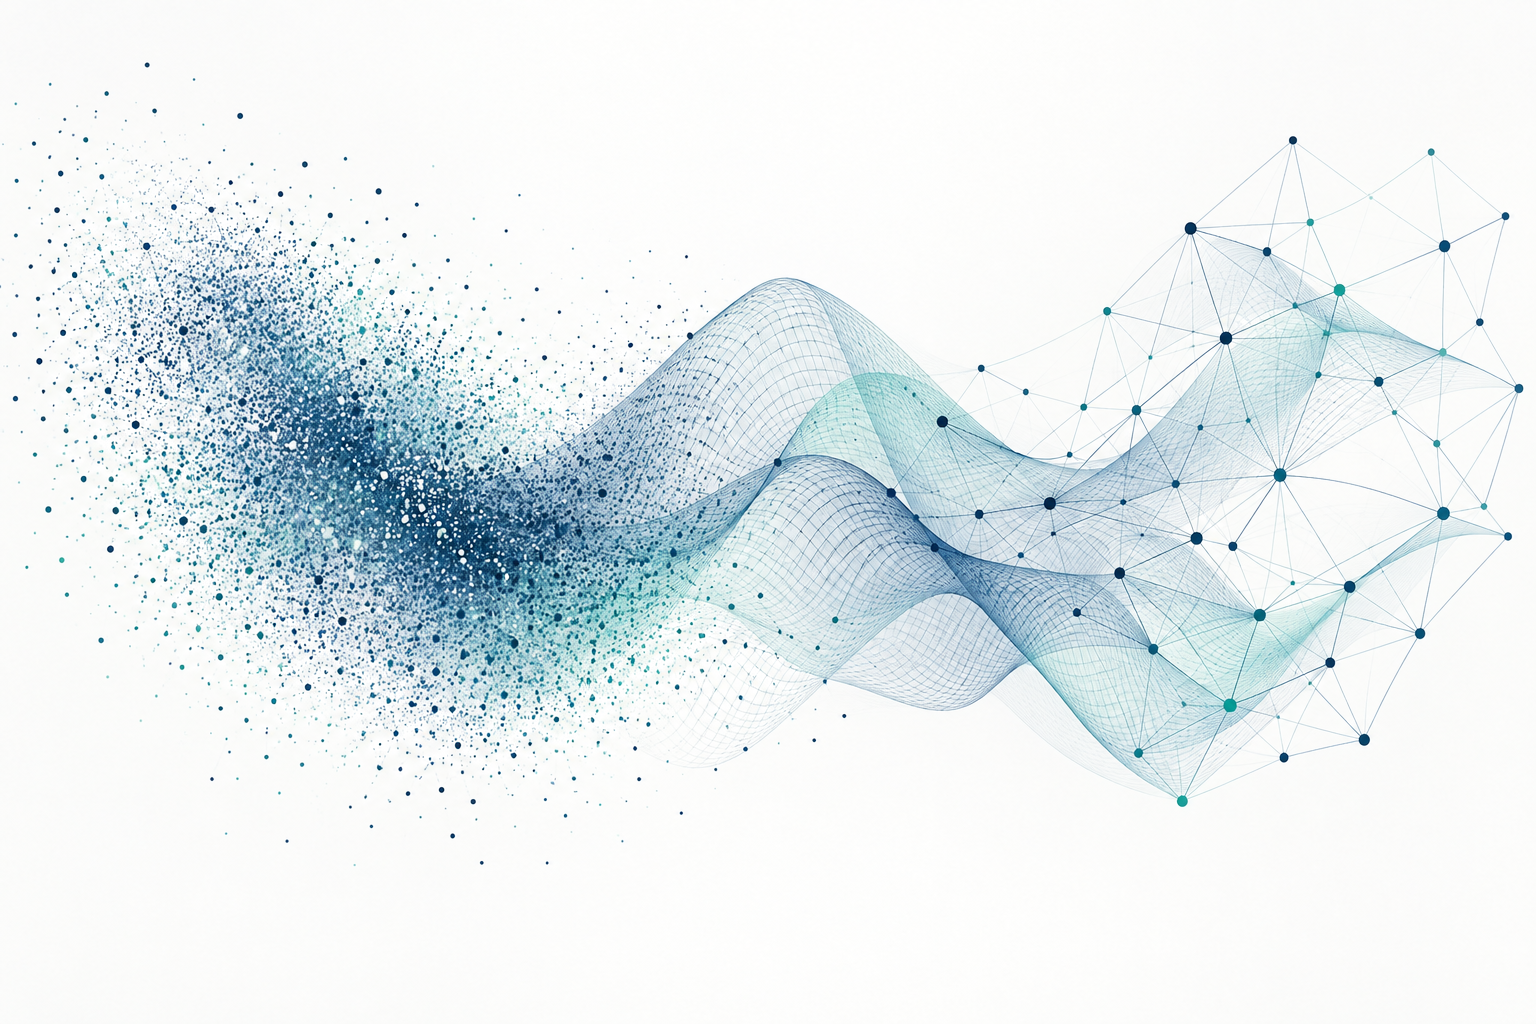
\includegraphics[width=\textwidth]{figures/cover.png}\par
\vfill
\noindent{\small\BookCity}\hfill{\small\BookYear}\par
\end{titlepage}
\restoregeometry
\setcounter{page}{1}\hypersetup{pageanchor=true}\thispagestyle{empty}
\begin{center}
{\small МИНИСТЕРСТВО НАУКИ И ВЫСШЕГО ОБРАЗОВАНИЯ\par РОССИЙСКОЙ ФЕДЕРАЦИИ\par}
\vspace{3mm}УНИВЕРСИТЕТ ИТМО\par
\vspace{23mm}{\large\BookAuthors\par}
\vspace{13mm}{\LARGE\bfseries\BookTitle\par}
\vspace{12mm}{\large ЛАБОРАТОРНЫЙ ПРАКТИКУМ\par}
\end{center}
\vfill\begin{center}\BookCity\par\BookYear\end{center}
\clearpage\thispagestyle{empty}
\begingroup\small\singlespacing
\noindent\BookAuthorsBib\ \BookTitle: лабораторный практикум. --- \BookCity: Университет ИТМО, \BookYear. --- \pageref*{LastPage}~с.
\par\bigskip
\noindent\textbf{Авторы:} \BookAuthorsFull.
\par\bigskip
\noindent\textbf{Рецензент:} \BookReviewer.
\par\bigskip
Практикум включает три работы: распознавание активности человека по признакам сигналов мобильных сенсоров; прогнозирование стоимости жилья полносвязной нейронной сетью; классификацию изображений цветов с использованием свёрточных сетей и переноса обучения. Для каждой работы приведены необходимые теоретические сведения, порядок выполнения, план исследования, контрольные точки и вопросы защиты.
\par\bigskip
Материал предназначен для студентов бакалавриата, изучающих дисциплину «Прикладной искусственный интеллект» и впервые знакомящихся с машинным обучением. Предполагаются навыки Python, работы с массивами и таблицами, знакомство со средним и производной. Основные понятия машинного обучения вводятся в самом практикуме. Сопровождающий комплект содержит учебные ноутбуки и код. Основные инструменты: scikit-learn, TensorFlow/Keras и PyTorch.
\par\bigskip
Особое внимание уделено корректному разделению данных, сопоставимости экспериментов, анализу ошибок и воспроизводимости результатов. Численные результаты опытов студент получает самостоятельно; в тексте приведены явно обозначенные расчётные примеры.
\par\bigskip
\noindent\textbf{Об Университете ИТМО}
\par\medskip
Университет ИТМО --- национальный исследовательский университет в Санкт-Петербурге. Его научные и образовательные направления включают информационные технологии и искусственный интеллект, фотонику, робототехнику, квантовые коммуникации, науки о жизни, искусство и научную коммуникацию. ИТМО участвует в программе «Приоритет-2030», развивает междисциплинарные исследования и индивидуальные образовательные траектории. С 2019 года университет самостоятельно присуждает учёные степени кандидата и доктора наук.
\par\bigskip
\noindent\copyright~Университет ИТМО, \BookYear\par
\noindent\copyright~Ким С.\,А., Евстафьев О.\,А., \BookYear
\endgroup

\clearpage\pagestyle{plain}
\begingroup\singlespacing\setlength{\cftbeforesecskip}{6pt}\tableofcontents\endgroup
\frontsection{Введение}
Практикум подготовлен по дисциплине «Прикладной искусственный интеллект». Искусственный интеллект объединяет методы решения задач, для которых нужны распознавание, прогнозирование или принятие решений. Машинное обучение --- одно из его направлений: модель находит закономерности по примерам. Три работы этого практикума посвящены именно машинному обучению и нейронным сетям на Python.

Практикум учит проходить полный цикл работы: понять данные, определить проверяемую задачу, построить модель, провести сопоставимые эксперименты и объяснить ошибки. Рабочий код служит инструментом исследования. Итог работы --- вывод, который можно проверить по сохранённым данным и результатам.

Три работы связаны общей логикой, но используют разные исходные данные и разные виды ответа. В первой модели получают уже вычисленные признаки сигналов и возвращают один из шести классов активности. Во второй сеть предсказывает непрерывную цену. В третьей признаки изображения формируются внутри свёрточной сети, а ответом служит вид цветка.

\begin{table}[H]\centering\small
\caption{Карта практикума}
\begin{tabularx}{\textwidth}{@{}>{\raggedright\arraybackslash}p{0.07\textwidth}>{\raggedright\arraybackslash}p{0.21\textwidth}Y Y@{}}
\toprule
№ & Задача & Главное новое умение & Проверяемый результат \\
\midrule
1 & Классификация активности & Сравнение алгоритмов; разделение по участникам & Отчёт по шести классам и матрица ошибок \\
2 & Регрессия стоимости & Подготовка смешанных признаков; обучение полносвязной сети & MAE/RMSE, анализ ошибок, таблица прогнозов \\
3 & Классификация цветов & Свёртки, перенос обучения, управление режимами модели & Сравнение трёх архитектур на одной валидации \\
\bottomrule
\end{tabularx}\end{table}

\subsection*{Входная подготовка}
Предшествующий курс машинного обучения не требуется. Нужны функции и коллекции Python, чтение таблиц в pandas, простые операции с массивами NumPy, среднее и представление о производной. Вектор можно сначала понимать как список чисел, матрицу --- как прямоугольную таблицу. Смысл новых понятий объясняется перед их использованием; формулы помогают проследить вычисление.

Начните с раздела «Первое знакомство с машинным обучением». Работы выполняйте по порядку: первая вводит сравнение моделей, вторая --- обучение нейросети, третья --- работу с изображениями. Обзор TabM и TabPFN-3 в конце практикума предназначен для дополнительного чтения.

\subsection*{Общий порядок работы}
\begin{enumerate}
\item Изучите исходные файлы и смысл меток. Проверьте размеры, пропуски, классы и идентификаторы.
\item Зафиксируйте разбиение, метрики, конфигурации и бюджет до сравнения результатов.
\item Выполните простой исходный вариант и проверьте контрольные точки.
\item Меняйте заранее выбранный фактор, сохраняйте результаты каждого опыта.
\item Объясните характерные ошибки и сформулируйте границы вывода.
\end{enumerate}

\begin{keybox}{Как читать примеры кода}
Сначала назовите вход и ожидаемый результат ячейки, затем выполните её и объясните полученное. Учебный модуль --- обычный файл Python с функциями: его можно открыть и прочитать. На первом проходе важнее понять роль функции; затем изучите нужные строки её реализации. Самостоятельная часть --- выбор, изменение модели и объяснение наблюдений.
\end{keybox}

\subsection*{Роль обучающей, валидационной и тестовой частей}
Обучающая часть определяет параметры модели и статистики преобразований. Валидация помогает выбрать настройки. Независимый размеченный тест используют после завершения выбора. Название файла само по себе не определяет его роль: в работе №\,1 \file{test.csv} содержит правильные ответы, а в работе №\,2 --- только признаки новых домов.

Подбор по одной и той же валидации постепенно приспосабливает к ней эксперимент. Поэтому в работах №\,2 и №\,3 результаты на валидации описывают качество выбора в данном опыте; они не объявляются независимой итоговой оценкой. В работе №\,1 предусмотрен отдельный финальный тест.

\frontsection{Первое знакомство с машинным обучением}
\label{sec:first-steps}
\subsection*{От примеров к правилу}
Предположим, в таблице записаны площадь, число комнат и известная цена нескольких домов. Мы хотим оценить цену другого дома. В машинном обучении правило прогноза настраивают по примерам с известным ответом. Эти примеры называются \textbf{обучающими данными}, а настраиваемое правило --- \textbf{моделью}.

\begin{table}[H]\centering\small
\begin{tabularx}{\textwidth}{@{}p{0.22\textwidth}Y@{}}
\toprule
Понятие & Пример и смысл \\
\midrule
Объект & Один дом; в таблице ему соответствует одна строка. \\
Признак & Известная характеристика дома, например площадь. \\
Целевой ответ & То, что требуется предсказать: здесь цена. \\
Выборка & Набор объектов, выделенный для определённой цели. \\
Прогноз & Ответ модели для конкретного объекта. \\
Обучение & Настройка модели по признакам и известным ответам. \\
\bottomrule
\end{tabularx}
\end{table}

При \textbf{регрессии} ответ --- число, например цена. При \textbf{классификации} ответ --- одна из заранее заданных категорий, например «ходит» или «сидит». Категории называют классами, а правильный класс объекта --- его меткой. Числовой код класса служит обозначением и не превращает задачу в регрессию.

Во всех трёх работах рассматривается \textbf{обучение с учителем}: для обучающих примеров известны правильные ответы. «Учитель» здесь означает наличие ответов в данных. Для нового объекта модель получает только те сведения, которые доступны при её применении.

\subsection*{Как читать обозначения}
Запись \(x_i\) обозначает признаки объекта с номером \(i\), \(y_i\) --- правильный ответ, \(\widehat y_i\) --- прогноз. Например, \(x_i=(80,3)\) может описывать площадь и число комнат. Символ \(f_\theta\) обозначает модель, а \(\theta\) --- её настраиваемые параметры:
\[
\widehat y_i=f_\theta(x_i).
\]
Эта формула читается так: «подать признаки объекта в модель и получить прогноз». В работе с изображениями признаки на входе --- значения пикселей; в работе с активностью --- уже вычисленные характеристики сигналов.

\clearpage
\subsection*{Почему нельзя проверять только на знакомых примерах}
Правило может хорошо отвечать на знакомые примеры и ошибаться на новых. Способность работать на новых объектах называют \textbf{обобщением}. Если модель слишком подстроилась под особенности обучения и хуже переносится на новые данные, говорят о \textbf{переобучении}.

Для организации проверки данные разделяют по ролям:
\begin{enumerate}
\item \textbf{Обучение (train):} настраиваем модель.
\item \textbf{Валидация (validation):} сравниваем варианты и выбираем настройки.
\item \textbf{Итоговый тест (test):} оцениваем выбранное решение, если есть отдельные данные с ответами, не использованные при выборе.
\end{enumerate}
Можно представить подготовку к экзамену: разобранные задачи помогают учиться, пробный вариант --- выбирать способ подготовки, новый экзаменационный вариант --- проверять результат. Это аналогия ролей, а не требование делить любой набор ровно на три файла.

\textbf{Утечка данных} возникает, если при обучении используется информация, которая по условиям проверки должна быть недоступна. Например, цена дома случайно оставлена среди признаков или средние для подготовки признаков вычислены с использованием валидации.

\subsection*{Что именно меняет экспериментатор}
\textbf{Параметры} модель находит при обучении: например, веса нейросети. \textbf{Гиперпараметры} задаёт исследователь: например, число соседей или ширину скрытого слоя. \textbf{Метрика} --- число, которым оценивают качество прогноза. \textbf{Исходная модель (baseline)} --- понятный вариант, с которым сравнивают изменения.

Под \textbf{протоколом} понимается заранее записанный порядок опыта: какие данные и разбиение используются, что меняется, какая метрика сравнивается. \textbf{Бюджет} ограничивает число запусков, эпох или время. \textbf{Seed} --- начальное состояние генератора случайных чисел: оно помогает повторить выбор разбиения и начальных весов, но не делает оценку качества безошибочной.

\begin{keybox}{Проверьте себя перед первой работой}
Выберите один дом или одно изображение. Назовите объект, доступные признаки и искомый ответ. Объясните, чем настройка модели отличается от проверки её прогноза. Если ответ пока неясен, вернитесь к этим определениям до запуска кода.
\end{keybox}

\frontsection{Подготовка среды и исходных материалов}
\ifdefempty{\CompanionURL}{}{%
\noindent Электронное приложение к практикуму:\par
\noindent\expandafter\url\expandafter{\CompanionURL}\par\medskip}
\subsection*{Структура файлов}
Держите исходные данные разных работ в отдельных каталогах. Файлы с одинаковыми именами относятся к разным задачам и не взаимозаменяемы.
\begin{lstlisting}[language={}]
project/
  code/                         # common teaching modules
  labs/
    01_classification/
      lab1_activity.ipynb
      data/                     # train.csv, test.csv
    02_regression/
      lab2_housing.ipynb
      data/                     # CSV and data_description.txt
    03_cnn/
      lab3_flowers.ipynb
      data/                     # five class folders
\end{lstlisting}

\noindent\begin{tabularx}{\textwidth}{@{}p{0.22\textwidth}Y@{}}
\toprule
Работа & Что должно быть в данных \\
\midrule
№\,1: активность & В обеих таблицах: числовые признаки, метка \file{Activity}, идентификатор участника (в коде --- \file{subject}). \\
№\,2: жильё & В обучающей таблице: \file{Id}, признаки и \file{SalePrice}; в таблице прогнозирования цены нет. Описание признаков находится в \file{data\_description.txt}. \\
№\,3: цветы & Пять каталогов видов с изображениями. Индексы классов определяются фактическим отображением \file{class\_to\_idx}. \\
\bottomrule
\end{tabularx}
\par\medskip
Преподаватель размещает выборки в папках работ или выдаёт их отдельно. Если в \file{data} пока только инструкция, добавьте необходимые файлы. Набор изображений указан в исходном задании: \href{https://www.kaggle.com/datasets/alxmamaev/flowers-recognition}{Flowers Recognition}. Количество строк, признаков и изображений определяйте по своей версии файлов.

\subsection*{Что такое ноутбук и как его запускать}
Ноутбук Jupyter (файл \file{.ipynb}) состоит из текстовых ячеек с пояснениями и ячеек Python. Выполняйте их сверху вниз. Переменные предыдущих ячеек остаются в памяти: если выполнить только нижнюю ячейку после изменения данных, можно случайно использовать старый результат. Перед итоговой проверкой перезапустите среду исполнения (kernel/runtime) и выполните все ячейки заново.

GitHub показывает содержимое ноутбука и хранит файлы; код исполняется в Jupyter Notebook или JupyterLab на компьютере студента либо учебном сервере. Для этого комплекта нужен весь проект с папкой \file{code}, а не только один \file{.ipynb}. В \file{START\_HERE.md} электронного приложения приведён порядок первого запуска. На GitHub сохраняйте себе копию материалов согласованной версии.

\subsection*{Программная среда}
Для работ №\,1 и №\,2 нужны Python, NumPy, pandas, scikit-learn и Matplotlib; для второго примера также TensorFlow/Keras. Для работы №\,3 нужны PyTorch, совместимая с ним torchvision и Pillow. Инструкции по проверенному локальному окружению находятся в \file{code/README.md}.

CPU --- центральный процессор компьютера. GPU --- ускоритель, который может быстрее выполнять многие операции нейросетей; его наличие не меняет смысла задания. В готовом учебном окружении сначала проверьте версии библиотек. При самостоятельной установке согласуйте версии Python, PyTorch, torchvision и доступного ускорителя по документации. Для работы на GPU нужна подходящая сборка библиотек.

\begin{lstlisting}
import sys
from importlib.metadata import version
print(sys.version)
for name in ("numpy", "pandas", "scikit-learn"):
    print(name, version(name))
\end{lstlisting}

В третьей работе ускоритель существенно сокращает время обучения. Проверка \file{torch.cuda.is\_available()} сообщает о доступности CUDA, а не о достаточном объёме памяти. Короткую проверку небольшого варианта можно выполнить на CPU; для сравнения тяжёлой исходной сети заранее оцените ресурсы.

\subsection*{Пути в ноутбуке}
Первая ячейка кода находит корень проекта по папкам \file{code} и \file{labs}, затем выбирает каталог своей работы. Поэтому путь \file{data/train.csv} ведёт к данным именно этой работы, а \file{runs} --- к её результатам. Запускать ноутбук можно из корня проекта или каталога работы. Сохраняйте структуру скачанного комплекта; для нового опыта выбирайте новое имя папки результатов.

\begin{keybox}{Перед запуском}
Проверьте, что открываете данные нужной работы; можете прочитать таблицу или изображение; понимаете смысл целевого ответа; знаете, какие файлы будут сохранены. Зафиксируйте версии библиотек и seed. Не сравнивайте результаты, полученные на незаметно разных разбиениях.
\end{keybox}

\practicalchapter{1}{Классификация}
\subsection{Постановка задачи и результат работы}
По признакам сигналов смартфона требуется определить вид активности человека. Объектом является временное окно измерений --- короткий фрагмент записи. Оно представлено вектором \(x_i\in\mathbb R^d\): списком из \(d\) числовых характеристик. Модель возвращает один класс:
\begin{equation}
\widehat y_i=f_\theta(x_i),\qquad y_i\in\{0,1,2,3,4,5\}.
\end{equation}
Числа обозначают категории: разность между метками не измеряет сходство движений. Устройство модели и её гиперпараметры студент выбирает и объясняет; в качестве сравнимого исходного набора ниже предложены три семейства алгоритмов.

\begin{table}[H]\centering\small
\caption{Словарь меток активности}
\begin{tabularx}{\textwidth}{@{}l l Y@{}}
\toprule
Код & Метка в файле & Смысл \\
\midrule
0 & \file{WALKING} & Ходьба \\
1 & \file{WALKING\_UPSTAIRS} & Ходьба вверх по лестнице \\
2 & \file{WALKING\_DOWNSTAIRS} & Ходьба вниз по лестнице \\
3 & \file{SITTING} & Сидение \\
4 & \file{STANDING} & Стояние \\
5 & \file{LAYING} & Положение лёжа \\
\bottomrule
\end{tabularx}\end{table}

\textbf{Результат сдачи:} таблица сравнения моделей на валидации, обоснованный выбор, итоговый \file{classification\_report} на тесте, матрица ошибок, визуализация сравнения и объяснение влияния гиперпараметров. По завершении работы вы должны уметь различать precision и recall, читать показатели по отдельным классам и объяснять, почему случайное разделение строк бывает недостаточным.

\subsection{От сигналов к признакам}
Описание исходного задания соответствует набору UCI Human Activity Recognition Using Smartphones. В первоисточнике 30 участников выполняли шесть действий со смартфоном на поясе; акселерометр и гироскоп регистрировали сигналы с частотой 50 Гц. Окна длиной 2,56 с содержали 128 отсчётов и перекрывались на 50\%. Из окна извлекались 561 признак во временной и частотной областях~\cite{har}. Число столбцов в учебной CSV-выгрузке проверяется отдельно.

Акселерометр измеряет ускорение, гироскоп --- угловую скорость. Фильтрация ослабляет шум; отделение низкочастотной составляющей помогает различать вклад гравитации и движения тела. Производные сигналов описывают скорость изменения, а евклидова норма объединяет три оси в скалярную величину. Преобразование Фурье показывает, как энергия сигнала распределяется по частотам. В этой работе не требуется заново реализовывать обработку сырых сигналов: используются готовые признаки.

\begin{table}[H]\centering\small
\caption{Как читать обозначения признаков исходного задания}
\begin{tabularx}{\textwidth}{@{}>{\raggedright\arraybackslash}p{0.42\textwidth}Y@{}}
\toprule
Обозначение & Что оно помогает описать \\
\midrule
\file{tBodyAcc}, \file{tGravityAcc}, \file{tBodyGyro} & Ускорение тела, гравитационная составляющая, угловая скорость; \file{t} обозначает временную область. \\
\file{Jerk}, \file{Mag}, \file{XYZ} & Изменение сигнала, его модуль, отдельные оси. \\
Префикс \file{f} & Представление в частотной области после БПФ. \\
\file{mean}, \file{std}, \file{mad}, \file{iqr} & Характеристики положения и разброса; точное определение проверяется по описанию признаков. \\
\file{max}, \file{min}, \file{sma}, \file{energy}, \file{entropy} & Экстремумы, совокупная амплитуда, энергия и характеристика распределения сигнала. \\
\file{arCoeff}, \file{correlation}, \file{angle} & Динамическая структура, связь сигналов, геометрическое соотношение векторов. \\
\file{maxInds}, \file{meanFreq}, \file{bandsEnergy}, \file{skewness}, \file{kurtosis} & Положение частотных компонентов, энергия полос и форма распределения. \\
\bottomrule
\end{tabularx}\end{table}

Не приписывайте признаку смысл только по имени. Например, величина \file{energy} зависит от принятого нормирования. Для последовательности \(a_1,\ldots,a_N\) удобный пример нормированной энергии --- \(N^{-1}\sum_i a_i^2\); это не то же самое, что сумма без деления на \(N\). В отчёте разберите два конкретных столбца своей таблицы.

\subsection{Разделение данных по участникам}
Если соседние окна одного человека попадают и в обучение, и в проверку, модель может воспользоваться индивидуальными особенностями и близостью записей. Результат тогда не обязательно переносится на нового участника. Для данного учебного протокола единица разделения --- \textbf{человек}, а единица классификации --- \textbf{окно сигнала}.

Сохраняйте внешний \file{test.csv} для итоговой проверки. Внутри \file{train.csv} выделите валидацию по идентификатору участника: примерно 20\% участников, фиксированный seed 40. \file{GroupShuffleSplit} определяет долю групп, поэтому доля строк может отличаться от 20\%~\cite{groupsplit}. Проверьте наличие всех шести классов в каждой части. Не выбирайте seed по наилучшей метрике.

\begin{keybox}{Три непересекающихся множества}
Участники обучения и валидации не пересекаются; участники внешнего теста отсутствуют в обеих этих частях. Столбцы \file{Activity} и \file{subject} не поступают в классификатор. Если идентификатора участника нет, нельзя утверждать, что проверена работа на новых людях: сначала уточните состав выгрузки и протокол.
\end{keybox}

Числовые признаки приводят к сопоставимому масштабу, например \(\widetilde x_j=(x_j-\mu_j)/s_j\). Среднее и масштаб вычисляются только на обучающей части. \file{Pipeline} связывает преобразование с моделью и предотвращает случайное применение нового scaler к проверочным объектам~\cite{pitfalls,scaler}.

\subsection{Три семейства классификаторов}
Каждый алгоритм строит своё правило ответа. Сначала разберите его идею словами, затем найдите в коде настройку, которая меняет это правило. Реализовывать алгоритмы библиотек самостоятельно не требуется.
\subsubsection*{Метод ближайших соседей}
Для нового вектора находятся \(k\) ближайших обучающих объектов; класс определяется голосованием. При евклидовом расстоянии
\begin{equation}
\rho(x,z)=\sqrt{\sum_{j=1}^d(x_j-z_j)^2}
\end{equation}
крупный масштаб одного признака может подавить вклад остальных. Поэтому в исходном сравнении KNN используется после стандартизации. Малое \(k\) делает ответ чувствительным к отдельным объектам; большое сильнее сглаживает границу. Существенны также способ взвешивания соседей и метрика расстояния~\cite{knn}.

\subsubsection*{Линейный метод опорных векторов}
При двух признаках линейную границу можно представить прямой на плоскости: точки по разные стороны получают разные ответы. Для большего числа признаков действует та же идея разделения. Метод опорных векторов (SVM) стремится получить границу с широким зазором между классами, допуская штрафуемые нарушения. Параметр \(C\) управляет компромиссом между регуляризацией и штрафом за нарушения разделения: уменьшение \(C\) усиливает регуляризацию --- ограничение сложности подгонки к обучению. Это не универсальное правило улучшения качества. В исходном сравнении используется \file{LinearSVC}; реализация линейного метода опорных векторов~\cite{linearsvc}.

\subsubsection*{Случайный лес}
Дерево последовательно задаёт вопросы о признаках, например «значение больше порога?», и в конце выдаёт класс. Случайный лес (Random Forest) объединяет ответы многих деревьев, обученных со случайным выбором объектов и доступных признаков. Ограничение глубины меняет сложность отдельных деревьев; число деревьев влияет на устойчивость ансамбля и вычислительные затраты. Масштабирование признаков для пороговых разбиений дерева обычно не требуется; для леса в предложенном протоколе scaler не добавляется~\cite{forest}.

\textbf{Гиперпараметры} задаются до обучения конкретной модели: \(k\), \(C\), глубина и число деревьев. Параметры, например коэффициенты линейной модели, определяются при \file{fit}. Изменение гиперпараметров требует нового обучения. Для контроля добавляется \file{DummyClassifier}, всегда предсказывающий самый частый класс обучения. Он показывает результат без анализа признаков: сравнение с ним помогает понять, чему научились остальные модели.

\subsection{Метрики и матрица ошибок}
Пусть \(C_{ij}\) --- число объектов истинного класса \(i\), отнесённых к классу \(j\). Строки матрицы ошибок соответствуют истине, столбцы --- прогнозу. Для класса \(c\):
\begin{align}
TP_c&=C_{cc}, & FP_c&=\sum_{i\ne c}C_{ic}, & FN_c&=\sum_{j\ne c}C_{cj},\\
P_c&=\frac{TP_c}{TP_c+FP_c}, & R_c&=\frac{TP_c}{TP_c+FN_c}, &
F_{1,c}&=\frac{2TP_c}{2TP_c+FP_c+FN_c}.
\end{align}
Precision отвечает на вопрос, какая доля предсказаний класса \(c\) верна. Recall показывает, какая доля настоящих объектов класса \(c\) найдена. F1 объединяет эти характеристики; высокая precision сама по себе не означает высокую полноту.
\begin{equation}
\mathrm{Accuracy}=\frac{\sum_c C_{cc}}{n},\qquad
\mathrm{MacroF1}=\frac{1}{6}\sum_{c=0}^{5}F_{1,c}.
\end{equation}
Macro-F1 придаёт каждому классу одинаковый вес. Weighted-F1 взвешивает классы по их численности; support --- число истинных объектов класса. Для выбора в этой работе используйте macro-F1 валидации, а accuracy и показатели по классам --- для дополнительного анализа~\cite{classification}.

\begin{keybox}{Пример для самопроверки}
Для класса «сидит» модель дала 10 положительных прогнозов: восемь верны, два относятся к другим классам; ещё четыре объекта класса «сидит» пропущены. Тогда precision равна \(8/10=0{,}8\), recall --- \(8/12\approx0{,}667\), F1 --- \(16/22\approx0{,}727\). Это вычислительный пример, не результат работы на данных курса.
\end{keybox}

При нулевом знаменателе метрика не определена обычной формулой. В коде \file{zero\_division=0} задаёт явное соглашение вывода; нулевой support или отсутствие предсказаний следует отметить. Нормирование матрицы по строкам помогает увидеть долю ошибок для каждого истинного класса, а абсолютные числа показывают объём наблюдений.

\subsection{Порядок выполнения}
\textbf{Первый проход:} прочитайте таблицу, назовите её служебные столбцы, затем выполните исходное сравнение без изменения настроек. Найдите одну строку результата и объясните её метрику. После этого переходите к исследованию гиперпараметров.

\subsubsection*{Шаг 1. Проверьте таблицы и метки}
Откройте файлы из \file{data}. Выведите размер таблиц, имена столбцов, число участников, распределение классов и наличие пропусков. Назовите два осмысленных признака. Не выбирайте входы срезом \file{values[:, :-2]}: положение служебных столбцов может измениться.
\begin{lstlisting}
from pathlib import Path
import pandas as pd
train = pd.read_csv(Path("data/train.csv"))
test = pd.read_csv(Path("data/test.csv"))
print(train.shape, test.shape)
print(train["Activity"].value_counts())
print(train["subject"].nunique(), test["subject"].nunique())
\end{lstlisting}

\subsubsection*{Шаг 2. Выделите валидацию}
Учебный модуль проверяет метки и признаки, исключает целевой столбец и идентификатор участника, затем выполняет групповое разделение. Если идентификатор называется иначе, укажите его через \file{group\_column}; не создавайте фиктивные номера участников из номеров строк.
\begin{lstlisting}
from lab1_utils import load_har, candidate_models, fit_validation
from lab1_utils import CLASSES, final_test, save_har_result
data = load_har("data", group_column="subject", seed=40)
print(data["Xtr"].shape, data["Xva"].shape)
print(data["training_subjects"], data["validation_subjects"])
\end{lstlisting}

\begin{keybox}{Контрольная точка}
Во входах нет \file{Activity} и идентификатора участника. Обучение, валидация и внешний тест содержат все шесть классов и разные группы людей. Валидация не участвует в вычислении параметров scaler. Столбцы теста приведены к порядку обучающих признаков по именам.
\end{keybox}

\subsubsection*{Шаг 3. Объясните выбор и выполните сравнение}
Сначала сформулируйте ожидаемое влияние гиперпараметров. В предлагаемом минимуме девять конфигураций с учётом константной модели. Допускается иной набор нескольких алгоритмов с сопоставимым и заранее определённым объёмом исследования.
\begin{table}[H]\centering\small
\caption{Исходный план сравнения классификаторов}
\begin{tabularx}{\textwidth}{@{}l l Y@{}}
\toprule
Обозначения & Модель & Меняемый параметр \\
\midrule
D0 & Dummy & Самый частый класс; ориентир без использования признаков \\
K3, K7, K15 & KNN & \(k\in\{3,7,15\}\); одинаковое масштабирование \\
S0.1, S1, S10 & LinearSVC & \(C\in\{0{,}1,1,10\}\); остальные настройки фиксированы \\
R8, RNone & Random forest & Глубина 8 или без ограничения; 200 деревьев \\
\bottomrule
\end{tabularx}\end{table}
\begin{lstlisting}
models = candidate_models(seed=40)
rows = []
for name, estimator in models.items():
    result = fit_validation(data, estimator)
    rows.append({"model": name, **result["metrics"],
                 "seconds_fit": result["seconds_fit"]})
comparison = pd.DataFrame(rows)
print(comparison.sort_values("macro_f1", ascending=False))
\end{lstlisting}

Этот цикл использует только обучение и валидацию. Сохраняйте предупреждения о сходимости; не скрывайте их общим отключением warnings. Если модель не сошлась, выясните причину и отдельно зафиксируйте изменённый бюджет или настройку.

\subsubsection*{Шаг 4. Визуализируйте и зафиксируйте выбор}
Постройте столбчатую диаграмму macro-F1 для всех конфигураций и отдельную диаграмму времени обучения. Не изображайте секунды и F1 как величины одной шкалы. Назовите худшие классы и предполагаемые причины ошибок. При близких результатах учитывайте сложность и время; не объявляйте небольшое различие устойчивым без повторной проверки.
\begin{lstlisting}
import matplotlib.pyplot as plt
comparison.plot.bar(x="model", y="macro_f1", legend=False)
plt.ylabel("Validation macro-F1")
plt.tight_layout()
\end{lstlisting}

\subsubsection*{Шаг 5. Выполните итоговый тест}
После выбора конфигурации переобучите её на всём \file{train.csv}; scaler внутри Pipeline также обучается заново. Только после этого получите прогноз \file{yhat} для \file{test.csv}. Пример ниже выбирает максимум macro-F1 валидации; окончательное объяснение выбора должно присутствовать в отчёте.
\begin{lstlisting}
selected = comparison.sort_values(
    ["macro_f1", "model"], ascending=[False, True]
).iloc[0]["model"]
final = final_test(data, models[selected])
yhat = final["prediction"]
print(pd.DataFrame(final["report"]).T)
save_har_result(data, comparison, selected, final, "runs/lab1_01")
\end{lstlisting}
Если результат теста оказался хуже ожиданий, опишите это как результат. Возвращение к выбору настроек после просмотра теста превращает его в ещё одну валидацию. Исходное требование сравнить несколько моделей выполняется на валидации; внешний тест оценивает уже выбранное решение.

\subsubsection*{Шаг 6. Разберите ошибки}
Постройте матрицу ошибок с одинаковым порядком шести меток. Выведите абсолютные числа и вариант с нормированием по строкам. Объясните хотя бы две заметные пары перепутанных действий; разделяйте наблюдение и гипотезу о его причине.
\begin{lstlisting}
from sklearn.metrics import ConfusionMatrixDisplay
ConfusionMatrixDisplay.from_predictions(
    data["ytest"], yhat, labels=range(6),
    display_labels=CLASSES, normalize="true", xticks_rotation=90
)
plt.tight_layout()
\end{lstlisting}

\subsection{Отчёт и вопросы защиты}
В отчёт включите паспорт файлов, состав разбиения по участникам, мотивацию выбора алгоритмов, таблицу всех конфигураций, две диаграммы, итоговый classification report и матрицу ошибок. Сохраните точные параметры модели, версии, seed и идентификаторы групп. Завершите выводом: какой вариант выбран, какие классы распознаются хуже и что можно проверить следующим опытом.

\begin{enumerate}
\item Что является объектом, признаком, целевой меткой и группой в этой работе?
\item Почему код активности нельзя трактовать как непрерывную величину?
\item Какую информацию дают акселерометр и гироскоп? Зачем нужны признаки частотной области?
\item Почему разбиение строк и разбиение участников проверяют разные условия применения?
\item Чем precision отличается от recall? Постройте собственный пример с FP и FN.
\item Как рассчитывается F1? Чем macro-F1 отличается от weighted-F1 и accuracy?
\item Чем гиперпараметр отличается от параметра обученной модели?
\item Как изменение \(k\), \(C\) и глубины деревьев повлияло на ваши результаты?
\item Почему scaler обучается только на обучающей части? Для каких моделей он особенно существенен?
\item Что означает нулевой support? Почему следует сохранять порядок меток в отчёте?
\item Почему нельзя выбрать победителя по внешнему тесту и затем назвать этот тест независимым?
\end{enumerate}

\begin{keybox}{Перед сдачей работы №\,1}
Есть сравнение нескольких моделей с вариациями гиперпараметров, визуализация, финальные предсказания и объяснение precision/recall/F1. Проверка отделена от подбора; \file{subject} не используется как входной признак. Указаны ограничения проверки на новых людях.
\end{keybox}

\practicalchapter{2}{Нейронные сети}
\subsection{Постановка задачи и результат работы}
По характеристикам дома необходимо предсказать его стоимость
\file{SalePrice}. Пусть \(x_i\) --- вектор подготовленных признаков,
\(y_i\) --- известная цена, а \(f_\theta\) --- модель с обучаемыми
параметрами \(\theta\). Тогда прогноз имеет вид
\begin{equation}
\widehat y_i=f_\theta(x_i),\qquad y_i\in\mathbb R_{>0}.
\end{equation}
Требуется подготовить данные, построить последовательную нейронную сеть,
исследовать её настройки, оценить результат на выделенной валидационной
части и получить прогнозы для домов из \file{test.csv}.

\textbf{Результат сдачи:} выполненный ноутбук, таблица экспериментов,
диагностические графики, обоснованный выбор конфигурации и таблица
\file{Id, SalePrice}. Отдельно сохраняются исходные данные эксперимента
и сведения, позволяющие его повторить.

\subsection{Обучение, валидация и данные для прогнозирования}
В исходном файле \file{train.csv} известны правильные ответы.
Разделим его строки на обучающую часть (80\%) и валидационную (20\%).
Первую используем для определения параметров преобразований и весов сети,
вторую --- для сравнения конфигураций. В \file{test.csv} ответов нет.

\begin{keybox}{Основное правило}
Медианы, средние, масштабы и словарь категорий определяются по обучающей
части. К валидации и новым домам применяются уже найденные преобразования.
В терминах scikit-learn: \file{fit\_transform} для обучения,
\file{transform} для остальных данных~\cite{pitfalls}.
\end{keybox}

Если сначала вычислить медиану по всему \file{train.csv}, а затем
разделить строки, в подготовку обучения попадёт информация о валидации.
Если отдельно закодировать категории в двух таблицах, один и тот же
числовой код может означать разные категории. Оба случая нарушают
условия корректного сравнения.

Случайное разделение подходит для учебного предположения о независимых
однородных наблюдениях. Для временного прогноза, повторных продаж одного
объекта или групп зависимых домов нужен другой способ разбиения.
Укажите применяемое предположение в отчёте.

Повторный выбор модели по одной валидации адаптирует решение к ней.
Полученные числа являются оценкой на использованном разбиении, а не
независимой финальной проверкой. Для такой проверки понадобилась бы
отдельная размеченная выборка, не участвовавшая в выборе настроек.

\subsection{Пропуски, категории и масштабирование}
Для числового признака в исходном варианте будем заменять пропуски
медианой обучающей части. Медиана меньше реагирует на отдельные очень
большие значения, чем среднее. Выбранное правило одинаково применяется
ко всем частям данных~\cite{imputer}.

Для категорий введём отдельное значение \file{\_\_missing\_\_}.
По описанию данных необходимо проверить, означает ли отсутствие записи
неизвестное значение или отсутствие самого объекта: например, гаража.
Автоматически отождествлять эти случаи нельзя. В исходном варианте
сохраняется фиксированное удаление пяти столбцов из задания:
\file{Alley}, \file{FireplaceQu}, \file{PoolQC}, \file{Fence},
\file{MiscFeature}. Это условие учебного сравнения, а не универсальное
правило обработки пропусков.

Категории без естественного порядка кодируем методом \textit{one-hot}:
каждой известной категории соответствует отдельный бинарный столбец.
Порядок столбцов задаётся кодировщиком, обученным один раз.
\file{handle\_unknown="ignore"} позволяет обработать ранее не встречавшуюся
категорию: её блок индикаторов будет нулевым~\cite{onehot}.
Это не даёт модели знаний о новой категории; её появление стоит отметить.

\begin{keybox}{Небольшой пример}
Для категорий \(A,B,C\) возможны коды
\(A\mapsto(1,0,0)\), \(B\mapsto(0,1,0)\),
\(C\mapsto(0,0,1)\). Замена их числами \(1,2,3\) навязывает
порядок и расстояния, которых в описании признака может не быть.
\end{keybox}

Числовые признаки приведём к сопоставимому масштабу:
\begin{equation}
\widetilde x_{ij}=\frac{x_{ij}-\mu_j}{s_j},
\end{equation}
где \(\mu_j,s_j\) вычислены только по обучающей части после заполнения
пропусков. Для постоянного признака реализация использует безопасный
масштаб 1. Масштабирование не делает признаки независимыми и не
превращает распределение в нормальное~\cite{scaler}.

В примере также стандартизуется целевая цена:
\begin{equation}\label{eq:target}
z_i=\frac{y_i-\mu_y}{s_y},\qquad
\widehat y_i=\mu_y+s_y\widehat z_i.
\end{equation}
Это помогает обучать сеть на числах умеренного масштаба.
Перед оценкой и сохранением прогноз возвращается к исходной цене.
Использовать среднюю цену валидационной части при обратном преобразовании
нельзя.

\subsection{Полносвязная нейронная сеть}
Нейрон полносвязного слоя вычисляет взвешенную сумму и применяет
функцию активации:
\begin{equation}
a_j=\sum_{k=1}^{d}w_{jk}x_k+b_j,\qquad h_j=\varphi(a_j).
\end{equation}
В матричной записи для слоя \(\ell\):
\begin{equation}
h^{(\ell)}=\varphi\!\left(W^{(\ell)}h^{(\ell-1)}+b^{(\ell)}\right),
\qquad h^{(0)}=\widetilde x.
\end{equation}
Сеть с одним скрытым слоем и линейным выходом задаёт
\begin{equation}
\widehat z=v^{\mathsf T}\varphi(W\widetilde x+b)+c.
\end{equation}
Реализация последовательности таких слоёв соответствует
\file{keras.Sequential}; полносвязный слой представлен
\file{Dense}~\cite{sequential,dense}.

\begin{figure}[htbp]
\centering\begin{tikzpicture}[>=Stealth,
  neuron/.style={circle,draw=accent,fill=light,minimum size=9mm},
  every node/.style={font=\small}]
\foreach \i/\label in {1/1,2/j,3/d}{
  \node[neuron] (x\i) at (0,-1.2*\i) {$x_{\label}$};}
\foreach \i/\label in {1/1,2/k,3/m}{
  \node[neuron] (h\i) at (4,-1.2*\i) {$h_{\label}$};}
\node[neuron] (y) at (8,-2.4) {$\widehat z$};
\foreach \i in {1,2,3}{\foreach \j in {1,2,3}{
  \draw[->,black!30] (x\i)--(h\j);}}
\foreach \i in {1,2,3}{\draw[->,black!45] (h\i)--(y);}
\node[align=center] at (0,0) {Подготовленные\\признаки};
\node[align=center] at (4,0) {Скрытый слой\\ReLU};
\node[align=center] at (8,0) {Линейный\\выход};
\end{tikzpicture}

\caption{Схема полносвязной сети. Показаны отдельные компоненты;
фактическое число входов определяется после предобработки.}
\label{fig:network}
\end{figure}

Входная размерность \(d\) равна числу подготовленных признаков.
Её нельзя произвольно менять при фиксированных данных.
В задании об изменении числа нейронов варьируется ширина
\textbf{первого скрытого полносвязного слоя}. Выходной слой содержит
один нейрон, поскольку для каждого дома предсказывается одно число.

У слоя с \(d\) входами и \(m\) нейронами имеется \(dm+m\)
обучаемых параметров. Для схемы \(d\to m\to1\) их всего
\begin{equation}
P=(d+1)m+(m+1).
\end{equation}
Например, при \(d=10\), \(m=8\) получаем \(P=97\).
Это вычислительная иллюстрация, а не характеристика файлов курса.
Сравните собственный расчёт с \file{model.count\_params()}.

\subsection{Функции активации}
Нелинейная активация позволяет сети представлять нелинейные зависимости.
Последовательность только линейных слоёв без активаций сводится к одному
аффинному преобразованию --- взвешенной сумме входов с добавлением смещения.

\noindent\begin{tabularx}{\textwidth}{@{}p{0.16\textwidth}p{0.28\textwidth}Y@{}}
\toprule
Активация & Формула & Особенность \\
\midrule
ReLU & \(\max(0,a)\) & Простая исходная активация скрытых слоёв;
на отрицательной полуоси производная равна нулю. \\
Sigmoid & \(1/(1+e^{-a})\) & Выход в \((0,1)\); в областях насыщения
производная мала. \\
Tanh & \(\tanh(a)\) & Выход в \((-1,1)\); также имеет области насыщения. \\
Линейная & \(a\) & Не ограничивает диапазон прогноза. \\
\bottomrule
\end{tabularx}

В основной конфигурации используем ReLU внутри сети и линейную функцию
на выходе~\cite{activations}. Sigmoid на выходе без согласованного
преобразования цели ограничила бы прогноз интервалом \((0,1)\).
Линейный выход для стандартизованной цели может принимать отрицательные
значения: это означает цену ниже \(\mu_y\), а не обязательно отрицательную
цену. Проверять допустимость нужно после обратного преобразования.

\subsection{Функции потерь и метрики регрессии}
Пусть на оцениваемой части имеется \(n\) объектов, а ошибка прогноза
\(e_i=y_i-\widehat y_i\). Определим
\begin{align}
\operatorname{MSE}&=\frac1n\sum_{i=1}^{n}e_i^2,\\
\operatorname{MAE}&=\frac1n\sum_{i=1}^{n}|e_i|,\\
\operatorname{RMSE}&=\sqrt{\frac1n\sum_{i=1}^{n}e_i^2}.
\end{align}
MAE и RMSE измеряются в единицах цены, MSE --- в квадрате этих единиц.
Квадратичная ошибка сильнее выделяет большие промахи. MAE придаёт
линейный вес абсолютной величине ошибки~\cite{losses}.

\begin{keybox}{Пример расчёта}
Пусть цены равны \((100,150,200)\), а прогнозы --- \((110,140,230)\)
в условных денежных единицах. Тогда
\(\operatorname{MAE}=50/3\approx16{,}67\),
\(\operatorname{MSE}=1100/3\approx366{,}67\),
\(\operatorname{RMSE}\approx19{,}15\).
Числа служат только для проверки понимания формул.
\end{keybox}

Дополнительно можно вычислить коэффициент детерминации
\begin{equation}
R^2=1-\frac{\sum_i(y_i-\widehat y_i)^2}
{\sum_i(y_i-\overline y)^2}.
\end{equation}
Здесь \(\overline y\) --- среднее по \textit{оцениваемой} части данных
в определении метрики, а не параметр предобработки.
Значение \(R^2\) может быть отрицательным; это не процент точных ответов.
При постоянной цели знаменатель равен нулю, и такая формула не определена
~\cite{metrics}.

\textbf{Функция потерь} задаёт то, что минимизирует обучение.
\textbf{Метрика} нужна для оценки и сравнения. При смене MSE на MAE
нельзя сравнивать сами значения \file{loss} как одну общую шкалу.
Во всех опытах сравнивайте одинаковые MAE и RMSE после возврата
к исходным ценам. Главным критерием выбора в этой работе назначается MAE
валидации; RMSE помогает увидеть крупные ошибки.

Для преобразования~\eqref{eq:target} справедливо
\(\operatorname{MAE}_y=s_y\operatorname{MAE}_z\) и
\(\operatorname{MSE}_y=s_y^2\operatorname{MSE}_z\).
Поэтому метрика в журнале обучения на стандартизованной цели и ошибка
в денежных единицах имеют разные численные значения.

\subsection{Обучение: градиент, эпоха и мини-выборка}
Обучение изменяет веса так, чтобы уменьшить среднюю потерю. Градиент
показывает, в какую сторону потеря растёт быстрее при малом изменении
параметров. Шаг в противоположную сторону помогает её уменьшить; величину
шага задаёт скорость обучения.
Для мини-выборки \(B_t\) шаг обычного градиентного метода имеет вид
\begin{equation}
\theta_{t+1}=\theta_t-\eta\nabla_\theta
\frac{1}{|B_t|}\sum_{i\in B_t}\ell(y_i,f_\theta(x_i)),
\end{equation}
где \(\eta>0\) --- скорость обучения. Производные вычисляются с
использованием цепного правила; последовательное распространение
производных от выхода сети к её входным слоям называют обратным
распространением ошибки.

\begin{keybox}{Один шаг обучения на простом примере}
Пусть \(\widehat y=wx+b\), \(x=2\), правильный ответ \(y=6\),
начальные \(w=1\), \(b=0\). Прогноз равен 2, а квадратичная потеря
\((\widehat y-y)^2=16\). Производные:
\[
\frac{\partial L}{\partial w}=2(\widehat y-y)x=-16,\qquad
\frac{\partial L}{\partial b}=2(\widehat y-y)=-8.
\]
При шаге \(0{,}01\) получаем \(w=1{,}16\), \(b=0{,}08\).
Новый прогноз равен \(2{,}4\), потеря --- \(12{,}96\): на этом шаге
она уменьшилась. В многослойной сети производные передаются через слои
по цепному правилу. Это учебный расчёт для одного объекта, не результат
обучения на домах.
\end{keybox}

\textbf{Итерация} в рассматриваемом режиме --- один шаг обновления весов
по мини-выборке. \textbf{Эпоха} --- проход по всей обучающей части.
Если в ней \(N\) строк и последний неполный пакет сохраняется, число
обновлений за эпоху равно \(\lceil N/b\rceil\), где \(b\) ---
\file{batch\_size}. При \(N=1000\), \(b=32\) это 32 обновления,
а за 10 эпох --- 320~\cite{training}.

Меньший пакет означает больше обновлений за эпоху и обычно более шумную
оценку градиента. Поэтому сравнение пакетов при одинаковом числе эпох
не является сравнением при одинаковом числе обновлений.
Слишком большая скорость обучения может привести к колебаниям или
расходимости; слишком малая --- к медленному улучшению.

В работе сравниваются SGD и Adam. SGD использует градиент текущего
пакета; Adam дополнительно накапливает оценки первого и второго моментов
градиента и адаптирует масштаб обновлений~\cite{sgd,adam}.
Одинаковая численная скорость обучения не означает одинаковые траектории
или одинаковую оптимальность настройки для двух алгоритмов.

\subsection{Переобучение и воспроизводимость}
\textbf{Регуляризация} ограничивает подгонку модели к особенностям
обучения. Например, штраф L2 добавляет к потере величину, растущую с
квадратами весов. Dropout во время обучения случайно отключает часть
выходов скрытого слоя, а при прогнозировании отключение не выполняется.
Эти приёмы меняют обучение и требуют проверки на валидации; в базовую
конфигурацию они не включены.

Переобучение можно заподозрить, если ошибка на обучении продолжает
уменьшаться, а на валидации перестаёт улучшаться или растёт.
По одной кривой нельзя автоматически установить причину: проверьте
подготовку данных, размер выборки, архитектуру и скорость обучения.

Дополнительный приём --- ранний останов: прекратить обучение после
заданного числа эпох без улучшения валидационной метрики и вернуть
лучшие сохранённые веса. В Keras это реализует
\file{EarlyStopping}~\cite{early}. В основных опытах с числом эпох
ранний останов выключен, чтобы сравнивать результаты после заданного
числа проходов. Его эффект исследуется отдельно.

Используйте одинаковое разбиение и исходный seed 40.
Начальные состояния генераторов задаются командой
\file{keras.utils.set\_random\_seed}.
В примере дополнительно включаются детерминированные операции, что уменьшает
дополнительную случайность вычислений~\cite{seed}.
Записывайте версии библиотек и устройство. Один seed не является
оценкой устойчивости и не гарантирует побитового совпадения на разных
программных и аппаратных платформах~\cite{determinism}.

\subsection{Порядок выполнения}
\textbf{Первый проход:} проследите путь одного дома от строки таблицы через подготовку признаков до прогноза цены. Выполните B0 и объясните MAE в денежных единицах. К сравнению десяти конфигураций переходите после проверки этого запуска.

\subsubsection*{Шаг 1. Изучите исходные таблицы}
Откройте обе таблицы и описание данных. Проверьте число строк и столбцов,
наличие \file{SalePrice} только в обучающем файле и уникальность
\file{Id} внутри каждого файла. Назовите два числовых и два
категориальных признака; объясните их смысл.

\begin{lstlisting}
from pathlib import Path
import pandas as pd

DATA_DIR = Path("data")
train_data = pd.read_csv(DATA_DIR / "train.csv")
test_data = pd.read_csv(DATA_DIR / "test.csv")
print(train_data.shape, test_data.shape)
print(train_data.head())
print(test_data.head())
print(train_data.isna().sum().sort_values(ascending=False).head(10))
\end{lstlisting}

\begin{keybox}{Контрольная точка 1}
В \file{train.csv} цена известна, в \file{test.csv} --- отсутствует.
\file{Id} нужен для связи прогноза с домом и не включается в признаки.
Пропущенную целевую цену нельзя заполнять медианой: такая строка не даёт
достоверного обучающего ответа.
\end{keybox}

\subsubsection*{Шаг 2. Выполните разделение и предобработку}
Сохраните фиксированное удаление пяти столбцов из исходного задания.
Отделите \file{SalePrice} и \file{Id}, затем разделите сырые строки
в отношении 80/20 с \file{random\_state=40}. Только теперь обучайте
преобразования. Готовая реализация находится в \file{lab2\_utils.py}.
Прочитайте функцию \file{prepare\_frames} и найдите в ней место,
где вычисляются обучающие статистики.

\begin{lstlisting}
import sys
sys.path.insert(0, "code")
from lab2_utils import load_course_data, constant_baselines

data = load_course_data(DATA_DIR, seed=40)
print(data["Atr"].shape, data["Ava"].shape, data["Atest"].shape)
print(data["removed_columns"])
print(data["feature_names"][:10])
\end{lstlisting}

Числовой конвейер объединяет заполнение медианой и стандартизацию.
Категориальный --- заполнение отдельной категорией и one-hot-кодирование.
\file{ColumnTransformer} применяет эти конвейеры к соответствующим
столбцам~\cite{columntransformer}. Признаки с целочисленными кодами
проверьте по словарю: тип хранения сам по себе не доказывает,
что признак количественный.

\begin{keybox}{Контрольная точка 2}
Три матрицы имеют одинаковое число столбцов и не содержат NaN или
бесконечностей. Пересечение \file{train\_ids} и
\file{validation\_ids} пусто. Объекты валидации не участвовали
в \file{fit} преобразований. Число входов сети равно
\file{data["Atr"].shape[1]}.
\end{keybox}

\subsubsection*{Шаг 3. Рассчитайте простые базовые прогнозы}
Для сравнения используйте константные прогнозы: среднюю и медианную цену
\textit{обучающей} части. Для каждого вычислите MAE и RMSE на валидации.

\begin{lstlisting}
baseline_table = pd.DataFrame(constant_baselines(data)).T
print(baseline_table)
\end{lstlisting}

Такая проверка показывает, даёт ли сложная модель пользу по сравнению
с решением, не использующим признаки. Нейросеть не обязана выигрывать:
если это не произошло, разберите причины и честно покажите результат.

\subsubsection*{Шаг 4. Постройте исходную нейросеть}
Создайте и проанализируйте последовательную модель. Исходная настройка:
один скрытый слой из 64 нейронов с ReLU, один линейный выход, Adam,
скорость обучения \(10^{-3}\), MSE. Входная размерность определяется
результатом предобработки.

\begin{lstlisting}
from tensorflow import keras

keras.utils.set_random_seed(40)
d = data["Atr"].shape[1]
model = keras.Sequential([
    keras.Input(shape=(d,)),
    keras.layers.Dense(64, activation="relu"),
    keras.layers.Dense(1, activation="linear"),
])
model.compile(
    optimizer=keras.optimizers.Adam(learning_rate=1e-3),
    loss="mse",
    metrics=[keras.metrics.MeanAbsoluteError(name="mae")],
)
model.summary()
\end{lstlisting}

Этот небольшой пример показывает работу API. Основное самостоятельное
задание --- изменить архитектуру, провести предусмотренные исследования
и объяснить результаты. Для своей реализации рассчитайте число параметров
вручную и проверьте его по сводке модели.

\subsubsection*{Шаг 5. Обучите модель и сохраните историю}
Передавайте в модель \file{Atr} и стандартизованную цель \file{ztr},
а валидационные данные задавайте явно. Не используйте переменную
\file{test\_data} в аргументе \file{validation\_data}.

\begin{lstlisting}
history = model.fit(
    data["Atr"], data["ztr"],
    validation_data=(data["Ava"], data["zva"]),
    epochs=100, batch_size=32, shuffle=True, verbose=0,
)
\end{lstlisting}

Сопровождающая функция \file{run\_experiment} объединяет создание
новой модели, обучение, обратное преобразование прогноза и расчёт метрик.
Используйте либо собственную последовательность шагов, либо эту функцию;
не обучайте две модели подряд по ошибке, принимая их за один опыт.

\begin{lstlisting}
from lab2_utils import run_experiment, plot_diagnostics

result = run_experiment(
    data, hidden=(64,), epochs=100, batch_size=32,
    optimizer="adam", learning_rate=1e-3,
    loss="mse", seed=40, early_stop=False,
)
print(result["metrics"])
fig = plot_diagnostics(data, result)
\end{lstlisting}

\subsubsection*{Шаг 6. Оцените качество и исследуйте ошибки}
Постройте три графика:
\begin{enumerate}
\item MAE обучения и валидации в зависимости от эпохи.
\item Предсказанная цена против фактической на валидации; добавьте прямую
\(\widehat y=y\), обозначающую идеальный прогноз.
\item Остаток \(e=y-\widehat y\) в зависимости от предсказанной цены;
добавьте горизонтальную линию \(e=0\).
\end{enumerate}
Во всех подписях укажите используемые единицы. По последним двум графикам
обсудите крупные промахи, систематическое завышение или занижение цены,
а также изменение разброса ошибки.

Выделите пять объектов с наибольшей абсолютной ошибкой и рассмотрите
их исходные характеристики. Не удаляйте их из валидации ради улучшения
метрики. Если предполагаете ошибку данных, сформулируйте проверяемую
гипотезу и укажите, каких сведений не хватает.

\begin{keybox}{Контрольная точка 3}
MAE и RMSE вычислены после обратного преобразования цели. Для каждой
конфигурации использованы те же валидационные объекты. У каждой кривой
указано, к какой модели и части данных она относится.
\end{keybox}

\subsubsection*{Шаг 7. Получите и сохраните прогноз}
После выбора конфигурации используйте её для всех строк
\file{test.csv}. В базовом варианте сохраняется модель, обученная на
80\% размеченных строк. Её прогнозы сопровождаются оценкой, полученной
на оставшихся 20\%.

\begin{lstlisting}
import numpy as np
from lab2_utils import save_experiment

preds = np.asarray(result["predictions"]).reshape(-1)
output = pd.DataFrame({
    "Id": data["prediction_ids"],
    "SalePrice": preds,
})
assert len(output) == len(test_data)
assert output["Id"].tolist() == test_data["Id"].tolist()
assert np.isfinite(output["SalePrice"]).all()
print("Negative prices:", int((output["SalePrice"] < 0).sum()))
save_experiment(data, result, "runs/baseline_01")
\end{lstlisting}

Не обрезайте отрицательные прогнозы незаметно. Сначала проверьте обучение
и обратное преобразование. Если выбирается правило постобработки,
обоснуйте его по валидации и одинаково примените к обоим наборам
прогнозов. Файл \file{predictions\_raw.csv} сохраняет исходные значения.

Допускается отдельное финальное переобучение на всём \file{train.csv}
после фиксации настроек. В этом случае нужно заново обучить
предобработку и сеть. Прежняя валидационная ошибка относится к прежней
модели: вычислять её на строках, включённых в финальное обучение,
как независимую оценку нельзя.

\Needspace{20\baselineskip}
\subsection{Выполнение на PyTorch}
Вы можете выполнить работу на PyTorch, сохранив те же разбиение,
предобработку, архитектуру, метрики и исследуемые факторы.
В обычном интерфейсе PyTorch обучение не выполняется вызовами
\file{model.compile()} и \file{model.fit()}: цикл записывается явно.
Минимальная последовательность действий внутри цикла~\cite{pytorch}:

\begin{lstlisting}
model.train()
for xb, yb in train_loader:
    optimizer.zero_grad()
    prediction = model(xb)
    loss = criterion(prediction, yb)
    loss.backward()
    optimizer.step()

model.eval()
with torch.no_grad():
    val_prediction = model(X_val_tensor)
\end{lstlisting}

В этом фрагменте загрузчик, модель, оптимизатор и тензоры требуется
создать самостоятельно. Проверьте, что прогноз и цель имеют одинаковую
форму \((b,1)\). Сочетание \((b,1)\) и \((b,)\) может привести
к нежелательному расширению размерностей при вычислении потерь.
В качестве функций потерь используйте \file{MSELoss} и \file{L1Loss}.
Результаты TensorFlow и PyTorch не обязаны совпадать при одинаковом seed:
сравнивайте соблюдение протокола и полученные метрики, а не побитовое
совпадение весов.

\subsection{Самостоятельное исследование гиперпараметров}
Перед запуском сформулируйте ожидаемое влияние каждого изменения.
Сравнивайте варианты с исходной конфигурацией, меняя один фактор за раз.
Для каждого запуска создавайте новую сеть и новый оптимизатор.
Продолжение обучения старой сети не является независимым опытом.

\begin{keybox}{Фиксированные условия}
Разделение 80/20; seed 40; одинаковая подготовка признаков и цели;
ReLU в скрытых слоях; линейный выход; скорость обучения \(10^{-3}\).
Основные опыты проводятся без раннего останова.
\end{keybox}

Таблица задаёт компактный план из десяти конфигураций. Это предложенный
учебный протокол, а не результаты подбора оптимальной модели.
Преподаватель может скорректировать бюджет до начала занятия.

\begin{table}[H]
\centering\small
\caption{План сравнения. В столбце «слои» указаны ширины скрытых слоёв.}
\begin{tabular}{@{}llllll@{}}
\toprule
Опыт & Слои & Эпохи & Пакет & Оптимизатор & Потеря \\
\midrule
B0 & 64 & 100 & 32 & Adam & MSE \\
W1 & 32 & 100 & 32 & Adam & MSE \\
W2 & 128 & 100 & 32 & Adam & MSE \\
D1 & 64, 32 & 100 & 32 & Adam & MSE \\
E1 & 64 & 30 & 32 & Adam & MSE \\
E2 & 64 & 200 & 32 & Adam & MSE \\
P1 & 64 & 100 & 16 & Adam & MSE \\
P2 & 64 & 100 & 64 & Adam & MSE \\
O1 & 64 & 100 & 32 & SGD & MSE \\
L1 & 64 & 100 & 32 & Adam & MAE \\
\bottomrule
\end{tabular}
\end{table}

\begin{enumerate}
\item \textbf{Ширина слоя.} Сравните B0, W1 и W2. Как изменились число
параметров, ошибка и разрыв между обучением и валидацией?
\item \textbf{Глубина.} Сравните B0 и D1. Объясните, какие изменения
вносит второй скрытый слой и оправдалось ли усложнение.
\item \textbf{Число эпох.} Сравните E1, B0 и E2. Покажите кривые
и определите, продолжалось ли улучшение к концу обучения.
\item \textbf{Размер мини-выборки.} Сравните P1, B0 и P2.
Рассчитайте число обновлений весов для каждого варианта и объясните,
почему одинаковое число эпох не означает одинаковый вычислительный опыт.
\item \textbf{Оптимизатор.} Сравните B0 и O1 при фиксированном шаге.
Вывод ограничьте этими настройками: он не доказывает общего превосходства
Adam или SGD при индивидуально подобранных скоростях обучения.
\item \textbf{Функция потерь.} Сравните B0 и L1 по одинаковым MAE
и RMSE в единицах цены. Разберите изменение крупных ошибок.
\end{enumerate}

\subsubsection*{Журнал результатов}
Для каждого опыта сохраните идентификатор, архитектуру, число параметров,
заданные и выполненные эпохи, размер пакета, оптимизатор, скорость
обучения, функцию потерь, seed, время обучения, MAE, RMSE и при
необходимости \(R^2\). Пример строки ниже содержит названия полей,
а не вымышленные результаты.

\begin{lstlisting}
row = {
    "experiment": "B0",
    **result["config"],
    **result["metrics"],
}
pd.DataFrame([row]).to_csv("experiment_B0.csv", index=False)
\end{lstlisting}

\subsubsection*{Как выбирать конфигурацию}
Сначала сравните MAE валидации, затем рассмотрите RMSE, сложность и
диагностические графики. Если разница мала, не объявляйте её устойчивым
преимуществом по одному запуску. Зафиксируйте, что обнаружено на данном
разбиении, и какая дополнительная проверка нужна.

Гиперпараметры не подбираются по \file{test.csv}: в нём нет правильных
ответов. В этой работе нет заданного универсального порога MAE или
требования обязательно превзойти все другие алгоритмы. Оценивается
корректность эксперимента и обоснованность выводов.

\subsubsection*{Дополнительные исследования}
По согласованию с преподавателем выполните одно расширение:
\begin{itemize}
\item включите ранний останов по MAE валидации и сравните с B0;
укажите фактическую длину обучения и правило возврата весов;
\item исследуйте влияние отдельной скорости обучения у SGD;
\item сравните фиксированное удаление пяти признаков с сохранением
их содержательно интерпретированных категорий;
\item повторите две выбранные конфигурации с несколькими заранее
заданными seed и покажите разброс на том же фиксированном разбиении.
\end{itemize}
Не смешивайте дополнительные опыты с исходной таблицей без указания,
какие условия изменились.

\clearpage
\subsection{Типичные ошибки и способы проверки}
\small
\begin{longtable}{@{}>{\raggedright\arraybackslash}p{0.27\textwidth}>{\raggedright\arraybackslash}p{0.30\textwidth}>{\raggedright\arraybackslash}p{0.35\textwidth}@{}}
\toprule
Наблюдение & Возможная причина & Проверка \\
\midrule\endhead
Разное число входных признаков & Кодировщик обучен отдельно на каждой
таблице & Один \file{fit} на обучении; одинаковые имена и порядок столбцов. \\
Подозрительно малая ошибка & Целевая цена попала в признаки или
статистики получены до разделения & Проверить список входов и место
вызова \file{fit}. \\
Ошибка обучения равна NaN & Остались NaN, бесконечности или обучение
расходится & Проверить массивы и цель; затем исследовать масштаб и шаг. \\
Прогнозы около нуля & Забыто обратное преобразование стандартизованной
цели & Применить тот же \file{target\_scaler}, который обучен на \(y_{train}\). \\
Плохое качество у дорогих домов & Большие ошибки на части диапазона,
редкие сочетания признаков & Изучить остатки и крупнейшие промахи;
не удалять их из валидации ради метрики. \\
Отрицательные исходные цены & Ошибочная шкала или неподходящее
поведение модели & Проверить обратное преобразование; обосновать
изменение модели или постобработку на валидации. \\
Результат меняется при повторе & Другое разбиение, случайная
инициализация, продолжение обучения & Сопоставить seed, версии,
идентификаторы строк и создание новой модели. \\
Ошибка размера тензоров в PyTorch & Цель имеет форму \((b,)\),
выход --- \((b,1)\) & Явно привести обе формы к \((b,1)\). \\
\bottomrule
\end{longtable}
\normalsize

\clearpage\subsection{Отчёт и защита работы №\,2}
\subsection*{Содержание отчёта}
\begin{enumerate}
\item ФИО, ИТМО ID, название и номер работы.
\item Цель, характеристика исходных данных и смысл используемых признаков.
\item Описание разбиения и предобработки: что удалено, как заполнены
пропуски, как обработаны категории и где вычислены статистики.
\item Архитектура исходной сети, размерности и расчёт числа параметров.
\item Таблица базовых прогнозов и всех выполненных конфигураций.
\item Кривые обучения, сравнение фактических и предсказанных цен,
анализ остатков и наиболее крупных ошибок.
\item Вывод о влиянии исследованных факторов и обоснование выбранной
конфигурации с указанием ограничений.
\item Пример итоговой таблицы прогнозов и описание файлов результата.
\item Список источников и параметры воспроизводимости.
\end{enumerate}

К отчёту приложите ноутбук с выполненными ячейками, исходный код изменений,
журнал опытов, истории обучения и прогнозы. Сохраняйте результаты всех
запланированных запусков, включая неудачные, с объяснением причины сбоя.
Полные CSV не требуется вставлять в PDF отчёта.

\subsection*{Критерии оценки}
\noindent\begin{tabularx}{\textwidth}{@{}p{0.28\textwidth}Y@{}}
\toprule
Критерий & Что необходимо показать \\
\midrule
Корректность данных & Разделение до обучения преобразований,
нет \file{Id} и цели во входах, согласованное кодирование. \\
Корректность модели & Подходящие вход и выход, согласованная потеря,
понимание количества параметров и процесса обучения. \\
Качество исследования & Сопоставимые опыты, сохранённые условия,
одинаковые метрики, объяснение результатов. \\
Анализ и вывод & Разбор ошибок и ограничений; вывод подтверждён
собственными наблюдениями. \\
Воспроизводимость & Данные, версии, разбиение, конфигурации и материалы
позволяют повторить опыт. \\
\bottomrule
\end{tabularx}

Баллы, пороги и правила повторной сдачи устанавливает преподаватель
по рабочей программе дисциплины. Исправный запуск кода без анализа
не демонстрирует всех результатов обучения этой работы.

\Needspace{9\baselineskip}
\subsection*{Контрольные вопросы}
\begin{enumerate}
\item Почему прогнозирование \file{SalePrice} относится к регрессии?
Чем признак отличается от класса и целевой переменной?
\item Для чего нужны обучение, валидация и \file{test.csv}?
На какой части допустим подбор гиперпараметров?
\item Почему нельзя отдельно обучать кодировщики категорий на обучающих
и новых данных? Приведите пример ошибки соответствия кодов.
\item Зачем масштабировать признаки и целевую цену? Как вернуть прогноз
к исходным единицам?
\item Что вычисляет полносвязный слой? Как найти число его параметров?
\item Почему входная размерность не меняется вместе с шириной скрытого слоя?
\item Что такое функция активации? Сравните ReLU, sigmoid и tanh.
Почему выход данной сети линейный?
\item Что такое эпоха и итерация? Сколько обновлений весов было
в вашем опыте и как на это повлиял \file{batch\_size}?
\item Что измеряют MSE, MAE и RMSE? В каких единицах они выражаются?
\item Почему при смене функции потерь нужно сохранять общие метрики сравнения?
\item Как ширина, глубина, число эпох, размер пакета и оптимизатор
повлияли на ваши результаты? Какие выводы поддерживаются данными?
\item Какие признаки переобучения вы наблюдали? Как работает ранний останов?
\item Почему лучший результат на одной валидации не гарантирует
лучшего результата на будущих домах?
\item Можно ли судить о качестве прогноза по первым строкам таблицы
\file{Id, SalePrice}, если правильная цена неизвестна?
\end{enumerate}

\begin{keybox}{Перед сдачей}
Убедитесь, что ноутбук выполняется последовательно из чистого состояния,
в отчёте есть собственные результаты всех обязательных сравнений,
а файл прогнозов содержит ровно те \file{Id} и в том же порядке,
что исходный \file{test.csv}.
\end{keybox}

\practicalchapter{3}{Свёрточные нейронные сети}
\subsection{Постановка задачи и результат работы}
Требуется классифицировать изображения пяти видов цветов: ромашки, одуванчики, розы, подсолнухи и тюльпаны. Исходное задание использует набор \href{https://www.kaggle.com/datasets/alxmamaev/flowers-recognition}{Flowers Recognition}. Изображения помещаются в каталоги \file{daisy}, \file{dandelion}, \file{rose}, \file{sunflower}, \file{tulip}; число файлов и соответствие индексов меткам нужно получить из своей копии данных.

\textbf{Обязательное сравнение сохраняет три части исходника:}
\begin{enumerate}
\item заданная свёрточная сеть, обучаемая с нуля;
\item предобученная свёрточная архитектура с новой головой классификации;
\item собственная архитектура студента, обучаемая с нуля.
\end{enumerate}
Необходимо объяснить устройство моделей, визуализировать результаты и сравнить качество при одинаковом разбиении. В пособии используется PyTorch, как и в коде исходного ноутбука. При выполнении на TensorFlow/Keras нужно явно перенести слои, режимы, предобработку и протокол, а не смешивать API двух фреймворков.

\textbf{Результат сдачи:} схема каждой архитектуры, число всех и обучаемых параметров, кривые обучения, таблица сравнения трёх моделей, матрицы ошибок, примеры прогнозов, сохранённые веса и описание воспроизводимого запуска.

\subsection{Изображение как тензор}
Тензор здесь --- многомерный массив чисел. Цветное изображение содержит три канала RGB: красный, зелёный и синий. В PyTorch пакет изображений имеет форму \((B,C,H,W)\): размер пакета, число каналов, высота, ширина. Для принятого входа это \((B,3,224,224)\). \file{ImageFolder} читает метки из имён каталогов и формирует \file{class\_to\_idx}; используйте это отображение и при обучении, и при выводе названий~\cite{imagefolder}.

Преобразование в тензор переводит обычные 8-битные RGB-пиксели в значения от 0 до 1. Затем выполняется нормализация каналов:
\begin{equation}
z_{c,h,w}=\frac{x_{c,h,w}-\mu_c}{\sigma_c},\qquad
x_{c,h,w}=\sigma_c z_{c,h,w}+\mu_c.
\end{equation}
В исходном примере используются \(\mu=(0{,}485,0{,}456,0{,}406)\) и \(\sigma=(0{,}229,0{,}224,0{,}225)\). Это фиксированные константы нормализации ImageNet, а не статистики, вычисленные по цветам. Для визуализации сначала выполните обратное преобразование; прямой \file{clip(0,1)} нормализованного тензора искажает цвета.

В исходном сравнении все модели получают \file{Resize((224,224))}, преобразование в тензор и одну нормализацию. Такое изменение размера может менять пропорции изображения. У весов ResNet18 есть собственный рекомендованный рецепт \file{weights.transforms()}: изменение размера и центральная обрезка~\cite{resnet18}. Это другой рецепт. Если сравниваете его с исходным, оформите отдельный опыт и применяйте выбранные правила одинаково к сравниваемым моделям.

\textbf{Аугментация} создаёт изменённые варианты обучающих изображений, например зеркальные отражения. Она помогает показать модели больше допустимых вариантов объекта, но преобразование должно сохранять его класс. В основном сравнении этой работы случайные преобразования выключены; их влияние можно исследовать отдельно. На валидации применяются фиксированные преобразования.

\subsection{Свёрточный слой}
Полносвязный слой рассматривает все входные координаты совместно. Свёрточный слой использует небольшой локальный участок и одни и те же веса в разных пространственных положениях. Для шага 1 и без дополнения границы один выходной канал вычисляется по правилу
\begin{equation}
a_{o,h,w}=b_o+\sum_{c=1}^{C_{in}}\sum_{u=0}^{k_h-1}\sum_{v=0}^{k_w-1}
W_{o,c,u,v}\,x_{c,h+u,w+v}.
\end{equation}
В \file{Conv2d} реализуется взаимная корреляция: ядро в этой записи не переворачивается. В терминологии нейронных сетей операцию традиционно называют свёрткой~\cite{conv2d}. Полученные карты признаков --- таблицы откликов фильтров в разных участках изображения --- проходят через нелинейность, например ReLU. Обучение определяет, какие локальные сочетания полезны для классификации.

\begin{keybox}{Маленький расчёт}
Для одной карты \(X=\left[\begin{smallmatrix}1&2&3\\4&5&6\\7&8&9\end{smallmatrix}\right]\), ядра \(K=\left[\begin{smallmatrix}1&0\\0&2\end{smallmatrix}\right]\), нулевого смещения и шага 1 без padding получается \(\left[\begin{smallmatrix}11&14\\20&23\end{smallmatrix}\right]\). Например, левый верхний элемент равен \(1+2\cdot5=11\). Найдите остальные элементы вручную.
\end{keybox}

Для размера входа \(H\), ядра \(k\), шага \(s\), padding \(p\) и dilation \(d\) высота выхода равна
\begin{equation}
H_{out}=\left\lfloor\frac{H+2p-d(k-1)-1}{s}+1\right\rfloor.
\end{equation}
Для ширины действует такая же формула. В этой работе \(d=1\). При \(k=3\), \(s=1\), \(p=1\) размер сохраняется. Для обычной свёртки без групп со смещением число параметров
\begin{equation}
P=C_{out}(C_{in}k_hk_w+1).
\end{equation}
Первый слой \(3\to32\) с ядром \(3\times3\) содержит \(32(3\cdot3\cdot3+1)=896\) параметров. Общие веса резко уменьшают число параметров относительно полносвязного соединения всех пикселей со всеми пространственными выходами.

\subsection{Pooling и устройство исходной сети}
\file{MaxPool2d(2,2)} выбирает максимум в каждом окне \(2\times2\) и уменьшает высоту и ширину вдвое для чётного входа. Он не обучает веса. Pooling уменьшает пространственную детализацию и стоимость следующих вычислений; это не означает полной устойчивости классификатора к любому сдвигу или повороту.

\begin{table}[H]\centering\small
\caption{Размерности исходной CNN при входе 224\(\times\)224}
\begin{tabularx}{\textwidth}{@{}p{0.58\textwidth}Y@{}}
\toprule
Последовательность операций & Форма без размера пакета \\
\midrule
Вход RGB & \(3\times224\times224\) \\
Conv \(3\to32\), ReLU, Conv \(32\to64\), ReLU, MaxPool & \(64\times112\times112\) \\
Conv \(64\to128\), ReLU, Conv \(128\to128\), ReLU, MaxPool & \(128\times56\times56\) \\
Conv \(128\to256\), ReLU, Conv \(256\to256\), ReLU, MaxPool & \(256\times28\times28\) \\
Flatten & \(200704\) \\
Linear, ReLU; Linear, ReLU; Linear & \(1024\to512\to5\) \\
\bottomrule
\end{tabularx}\end{table}

Все свёртки в таблице имеют ядро 3, шаг 1 и padding 1. Полная реализация \file{original\_cnn()} в учебном модуле сохраняет размеры слоёв полученного ноутбука. Flatten только меняет представление тензора: он не извлекает новые признаки.

\begin{keybox}{Почему нужно заранее оценить память}
Слой \(200704\to1024\) содержит \(205\,521\,920\) параметров со смещением. Вся исходная сеть --- \(207\,175\,365\). Только веса float32 занимают около 0,77 GiB. Веса, градиенты и два состояния Adam суммарно требуют около 3,09 GiB, ещё без активаций и временных буферов. Это расчёт по архитектуре, а не измерение пикового расхода памяти.
\end{keybox}

Для собственной модели полезно исследовать глобальное усреднение карт. В примере оно выполняется слоем \file{AdaptiveAvgPool2d(1)}. Этот слой превращает \(C\times H\times W\) в \(C\times1\times1\), после чего компактная голова предсказывает пять классов. Это уменьшает число параметров, но меняет модель и не гарантирует лучшего качества. В комплекте дан небольшой пример; самостоятельная архитектура должна содержать обоснованное собственное изменение.

\subsection{Логиты, cross-entropy и обучение}
Последний слой выдаёт пять логитов \(z_1,\ldots,z_5\) --- оценок классов, которые могут быть любыми вещественными числами. Softmax превращает их в положительные числа с суммой 1. Вероятности softmax определяются как
\begin{equation}
p_c=\frac{e^{z_c}}{\sum_{j=1}^{5}e^{z_j}},\qquad
L=-\frac1B\sum_{i=1}^{B}\log p_{i,y_i}.
\end{equation}
\file{CrossEntropyLoss} принимает исходные логиты формы \((B,5)\) и целочисленные индексы классов формы \((B,)\) с типом \file{torch.long}. Отдельный Softmax перед этой функцией не нужен~\cite{crossentropy}. Для выбора класса достаточно \file{logits.argmax(dim=1)}; наибольший логит и наибольшая вероятность имеют один индекс. Вероятность softmax сама по себе не является проверенной уверенностью модели.

Итерация обучения включает обнуление градиентов, прямой проход, вычисление потери, обратный проход и шаг оптимизатора. При проверке обратный проход и шаг отсутствуют. \file{model.eval()} переключает поведение слоёв, а отключение градиентов снижает затраты на вычислительный граф: это разные операции.

Метрики считают заново для каждой эпохи и каждой фазы. Средняя потеря должна учитывать размер последнего пакета:
\begin{equation}
L_{epoch}=\frac{\sum_b n_b L_b}{\sum_b n_b}.
\end{equation}
Например, для пакетов из 32 и 8 изображений нельзя брать простое среднее двух потерь. Accuracy считают по всем правильным ответам фазы, macro-F1 --- по всем её меткам и прогнозам, а не как невзвешенное среднее F1 пакетов.

\subsection{Перенос обучения и заморозка}
Предобученная сеть уже получила веса на другой задаче. Основную часть сети, преобразующую изображение в признаки, называют \textbf{извлекателем признаков (backbone)}. Завершающий блок, переводящий эти признаки в ответы нашей задачи, называют \textbf{головой классификации (head)}. В переносе обучения её признаки применяются к новому набору. В исходном варианте оставляют фиксированный извлекатель признаков и обучают новую голову; при \textbf{дообучении (fine-tuning)} дополнительно изменяют часть предобученных слоёв. Эти режимы нужно различать в отчёте~\cite{transfer}.

Пример использует ResNet18 с явно указанными весами \file{IMAGENET1K\_V1}. Основой сети служат остаточные блоки: к преобразованию входа добавляется путь, передающий сам вход. Если размеры совпадают, блок имеет вид \(h_{next}=\operatorname{ReLU}(F(h)+h)\); при изменении размеров применяется согласующее преобразование короткого пути. Четыре группы блоков используют 64, 128, 256 и 512 каналов; после глобального усреднения заменяется слой \file{fc} на \(512\to5\)~\cite{resnetpaper,resnet18}.

\file{requires\_grad=False} исключает параметры из расчёта их градиентов. Новая голова создаётся после заморозки и остаётся обучаемой; её параметры включаются в оптимизатор. BatchNorm нормализует промежуточные значения в сети. У него есть также текущие средние и дисперсии --- сохраняемые служебные значения (буферы), изменяющиеся в режиме обучения~\cite{batchnorm}. Для полностью фиксированного извлекателя в данном протоколе backbone работает в \file{eval}, а новая голова --- в \file{train}. Простого общего вызова \file{model.train()} здесь недостаточно.

Сравнение с обучением с нуля учитывает дополнительный ресурс: веса ResNet получены на внешних данных. Поэтому вывод относится к практическим стратегиям обучения при указанном предобучении; это не сравнение одной лишь архитектуры при одинаковом объёме исходной информации.

\subsection{Подготовка изображений и разбиение}
\textbf{Первый проход:} откройте одно изображение, найдите его метку и форму тензора, затем проверьте размер выхода модели. До длительного обучения оцените память и выполните короткий пробный проход. Он проверяет запуск, но ещё не показывает качество обучения.

\subsubsection*{Шаг 1. Изучите набор и проверьте ресурсы}
Выведите пять классов, число изображений каждого класса и несколько исходных примеров. Проверьте читаемость файлов, размеры, цветовые каналы и дубликаты. Не задавайте число изображений по чужому описанию: оно зависит от версии выгрузки. Выберите устройство и запишите его в отчёте.
\begin{lstlisting}
import torch
from lab3_utils import prepare_flowers, seed_everything
from lab3_utils import original_cnn, transfer_resnet18, compact_example
from lab3_utils import fit_flowers, plot_learning, parameter_counts
seed_everything(0)
device = "cuda" if torch.cuda.is_available() else "cpu"
print(device)
\end{lstlisting}

\subsubsection*{Шаг 2. Зафиксируйте одну валидацию}
Исходный ноутбук выделяет 1000 изображений. В исправленном варианте это ориентир размера валидации; точные копии файлов объединяются по SHA-256 и попадают в одну часть. Поэтому фактическое число проверочных изображений может отличаться от 1000. \file{split.csv} сохраняет итоговое распределение. Групповое разделение не гарантирует одинаковые пропорции классов: выведите их и проверьте наличие всех пяти классов в обеих частях.
\begin{lstlisting}
data = prepare_flowers("data", validation_target=1000,
                       seed=0, image_size=224, augment=False)
print(data["class_to_idx"])
print(data["inventory"].groupby(["split", "target"]).size())
print(data["config"])
\end{lstlisting}

Хеши находят побайтовые копии. Снимки одной сцены после повторного сжатия, обрезки или изменения размера могут иметь разные хеши. Если такие серии известны, их также следует объединить до разделения. Совпадающие файлы с разными метками требуют проверки разметки. Не исправляйте конфликты только ради улучшения метрики.

Обучающий и проверочный наборы создаются как отдельные \file{ImageFolder} с одним списком файлов и разными подмножествами. При дополнительном опыте со случайным отражением оно применяется только к обучению. Замена \file{transform} у общего объекта под двумя \file{Subset} изменила бы обе части одновременно.

\begin{keybox}{Контрольная точка 1}
Пакет имеет форму \((B,3,224,224)\), метки --- целочисленный вектор длины \(B\) со значениями от 0 до 4. Известно отображение индексов в имена. Обучение и валидация не пересекаются по файлам и точным дубликатам. Все три архитектуры используют одно сохранённое разбиение.
\end{keybox}

\subsection{Обучение и исследование архитектур}
\subsubsection*{Шаг 3. Разберите и обучите заданную CNN}
Выпишите размеры тензоров после свёрток и pooling, проверьте вход первого Linear и число параметров. Создайте новую модель, затем оптимизатор. Функция ниже использует Adam с явно переданным шагом, десять эпох и пакет 32. Её код доступен в \file{lab3\_utils.py}; найдите места сброса метрик, переключения режима и выбора сохранённых весов.
\begin{lstlisting}
seed_everything(0)
model = original_cnn()
print(parameter_counts(model))
result_original = fit_flowers(
    model, data, "runs/lab3_original_01", epochs=10,
    batch_size=32, learning_rate=1e-3, seed=0, device=device
)
\end{lstlisting}

Перед полным запуском проверьте один пакет. Если памяти недостаточно, уменьшите пакет и заново зафиксируйте общий протокол для всех трёх моделей. Уменьшение разрешения у исходной сети потребует изменения первого Linear; это уже другая архитектура и должно быть указано. Не заносите ошибку памяти в таблицу качества как нулевую accuracy.

\subsubsection*{Шаг 4. Примените перенос обучения}
Выберите предобученную архитектуру, прочитайте её описание и определите слой классификатора. Пример ниже конкретизирует ResNet18. Порядок важен: сначала заморозка старых параметров, затем создание новой головы.
\begin{lstlisting}
from torchvision import models
from torch import nn
weights = models.ResNet18_Weights.IMAGENET1K_V1
model = models.resnet18(weights=weights)
for p in model.parameters():
    p.requires_grad = False
model.fc = nn.Linear(model.fc.in_features, 5)
model.frozen_backbone = True
for name, p in model.named_parameters():
    if p.requires_grad:
        print(name, p.shape)
\end{lstlisting}
Вывод должен содержать только \file{fc.weight} и \file{fc.bias}. Для головы \(512\to5\) обучается \(512\cdot5+5=2565\) параметров. При первом использовании веса могут загружаться из сети; \file{weights=None} создаёт случайную инициализацию и не является переносом обучения.

Фабрика \file{transfer\_resnet18()} выполняет эти действия и сохраняет обозначение весов в метаданных. Используйте новую модель и новый каталог опыта:
\begin{lstlisting}
seed_everything(0)
model = transfer_resnet18(pretrained=True)
result_transfer = fit_flowers(
    model, data, "runs/lab3_transfer_01", epochs=10,
    batch_size=32, learning_rate=1e-3, seed=0, device=device
)
\end{lstlisting}
В режиме фиксированного извлекателя проверьте, что параметры backbone и статистики BatchNorm не меняются после шага. Если исследуете fine-tuning, явно укажите размороженные слои, режим BatchNorm и новый оптимизатор. Не представляйте этот дополнительный опыт как тот же режим заморозки.

\subsubsection*{Шаг 5. Создайте собственную архитектуру}
Предложите изменение, связанное с проверяемой гипотезой: уменьшение головы, другая ширина блоков, изменение глубины, регуляризация или иной способ агрегирования карт. Нарисуйте последовательность слоёв, рассчитайте формы и число параметров. Выход обязан иметь пять логитов. Маленькая модель ниже иллюстрирует конструкцию с глобальным усреднением:
\begin{lstlisting}
student_model = nn.Sequential(
    nn.Conv2d(3, 16, 3, padding=1), nn.ReLU(), nn.MaxPool2d(2),
    nn.Conv2d(16, 32, 3, padding=1), nn.ReLU(), nn.MaxPool2d(2),
    nn.Conv2d(32, 64, 3, padding=1), nn.ReLU(),
    nn.AdaptiveAvgPool2d(1), nn.Flatten(), nn.Linear(64, 5)
)
\end{lstlisting}

\textbf{Самостоятельная часть:} внесите как минимум одно осмысленное структурное изменение относительно данного примера и объясните ожидаемый эффект. Простое копирование \file{compact\_example()} не считается разработкой своей архитектуры. Обучите свой вариант с тем же разбиением и основным бюджетом. Зафиксируйте seed \emph{до} создания слоёв, а не только перед вызовом функции обучения.

\subsection{Сравнение, визуализация и сохранение}
\subsubsection*{Шаг 6. Соберите сопоставимые результаты}
Основной протокол: RGB 224\(\times\)224, фиксированная нормализация, без случайной аугментации, seed 0, Adam с шагом \(10^{-3}\), пакет 32, десять эпох. Для каждой модели создаются новые загрузчики с тем же начальным seed. Выбирается эпоха с наибольшим macro-F1 валидации; при равенстве сохраняется более ранняя. Это одинаковое правило выбора, но не одинаковый объём предобучения.

\begin{table}[H]\centering\small
\caption{Что должно быть в итоговой таблице CNN}
\begin{tabularx}{\textwidth}{@{}p{0.30\textwidth}Y@{}}
\toprule
Группа полей & Содержание \\
\midrule
Модель & Имя, схема, число всех и обучаемых параметров; исходные веса \\
Обучение & Разбиение, seed, эпохи, пакет, оптимизатор, шаг, размер входа, аугментация \\
Результат & Лучшая эпоха, loss, accuracy и macro-F1 одной валидации \\
Ресурсы & Устройство, измеренное время с указанием границ измерения; при измерении --- пиковая память \\
Вывод & Какие классы и случаи улучшились или ухудшились; ограничения сравнения \\
\bottomrule
\end{tabularx}\end{table}

В модуле время включает обучение, валидацию и запись контрольных точек; оно не включает первоначальную загрузку предобученных весов и подготовку набора. Не сравнивайте его с измерением только одного прямого прохода. Одинаковое число эпох также не означает одинаковое число операций для разных сетей.

\subsubsection*{Шаг 7. Постройте графики и исследуйте прогнозы}
Для каждой модели покажите train/validation loss и macro-F1 по эпохам, а затем общую диаграмму результатов трёх архитектур. Сохраните матрицы ошибок и classification report по пяти классам. Используйте одинаковые оси и порядок меток, подпишите доли или проценты.
\begin{lstlisting}
fig = plot_learning(result_transfer)
fig.savefig("runs/lab3_transfer_01/curves.pdf", bbox_inches="tight")
\end{lstlisting}

Покажите девять заранее определённых изображений валидации либо все, если их меньше: истинный и предсказанный класс, восстановленные цвета. Дополнительно разберите несколько ошибок; не выбирайте только удачные картинки. Фрагмент демонстрирует корректный прогноз одного нормализованного изображения:
\begin{lstlisting}
from lab3_utils import denormalize
import matplotlib.pyplot as plt
index = int(data["validation_indices"][0])
image, label = data["validation_dataset"][index]
model = result_transfer["model"]
model.eval()
with torch.no_grad():
    logits = model(image.unsqueeze(0).to(device))
predicted = int(logits.argmax(1).item())
plt.imshow(denormalize(image).permute(1, 2, 0))
plt.title(f"True: {data['classes'][label]}; predicted: {data['classes'][predicted]}")
plt.axis("off")
\end{lstlisting}

\subsubsection*{Шаг 8. Сохраните воспроизводимый комплект}
Каждая архитектура получает свой каталог. Основные файлы:
\begin{itemize}
\item \file{split.csv} --- список изображений и разбиение;
\item \file{history.csv} --- история обучения по эпохам;
\item \file{best\_weights.pth} --- выбранные веса;
\item \file{manifest.json} --- параметры и результаты опыта;
\item \file{architecture.txt} --- текстовое описание модели.
\end{itemize}
Также сохраняются прогнозы, отчёт и матрица ошибок. Приложите исходный код собственной архитектуры. Для восстановления нужны совместимое определение модели, те же преобразования и тот же словарь классов, а не только файл весов.

Валидация используется для выбора эпохи и сравнения архитектур. Поэтому её лучший результат нельзя назвать независимой оценкой на новых фотографиях. Дополнительный финальный тест требует отдельного набора, не использованного при этих решениях.

\subsection{Контрольные вопросы и критерии готовности}
\begin{enumerate}
\item Чем CNN отличается от полносвязной сети по связям, параметрам и работе с пространством?
\item Что задают kernel size, stride, padding, входные и выходные каналы? Рассчитайте размер выхода одного слоя.
\item Как работают свёртка и pooling в исходной сети? Какие из них имеют обучаемые параметры?
\item Почему первый Linear исходной архитектуры требует так много памяти?
\item Что такое логиты? Почему перед CrossEntropyLoss не добавляется Softmax?
\item Зачем нужны одновременно eval и отключение градиентов?
\item Что такое предобучение, transfer learning и fine-tuning? Откуда взяты веса выбранной модели?
\item Как устроена выбранная предобученная архитектура? Для ResNet объясните короткий путь и сложение в блоке.
\item Что делает requires\_grad? Почему заморозка параметров не равна заморозке статистик BatchNorm?
\item Какое изменение вы внесли в собственную сеть и какую гипотезу проверяли?
\item Почему нельзя накапливать счётчики разных эпох или усреднять F1 пакетов как F1 всего набора?
\item Как корректно показать нормализованное изображение? Почему clip без обратной нормализации неверен?
\item Что можно и чего нельзя заключить из сравнения с предобученной сетью?
\end{enumerate}

\begin{keybox}{Перед сдачей работы №\,3}
Обучены и сопоставлены все три требуемые архитектуры; объяснены свёртка, pooling, перенос обучения и заморозка. Есть собственное изменение модели, общая таблица, графики и анализ ошибок. Преобразования и разбиение согласованы, метрики относятся к отдельным эпохам, а не ко всему предыдущему обучению.
\end{keybox}

\frontsection{Общие требования к отчёту и рекомендации преподавателю}
\subsection*{Структура отчёта}
Для каждой работы укажите ФИО, ИТМО ID, номер и название. Далее приведите цель, описание исходных данных, протокол разбиения, исходную модель, план опытов, результаты и выводы. Полные таблицы данных и многотысячные листинги не требуется вставлять в PDF: они передаются отдельными файлами. В тексте должны оставаться сведения, необходимые для понимания и проверки вывода.

\begin{enumerate}
\item \textbf{Постановка.} Что предсказывается, какие данные доступны и какая ошибка существенна.
\item \textbf{Протокол.} Как получены части данных, что обучалось только на training, по какой метрике выбирались настройки.
\item \textbf{Модель.} Принцип работы, архитектура или алгоритм, параметры опыта и мотивация выбора.
\item \textbf{Результаты.} Таблица всех запланированных опытов, необходимые графики, разбор ошибок.
\item \textbf{Вывод.} Наблюдение, возможное объяснение, ограничение и следующий проверяемый шаг.
\end{enumerate}

\subsection*{Критерии оценивания}
\begin{table}[H]\centering\small
\begin{tabularx}{\textwidth}{@{}p{0.25\textwidth}Y@{}}
\toprule
Критерий & Наблюдаемый признак выполнения \\
\midrule
Данные & Известны признаки и цель; нет утечки, перепутанных выборок и неверных меток. \\
Модель & Студент объясняет алгоритм, размерности, потери и изменяемые настройки. \\
Эксперимент & Сравнения воспроизводимы; сохранены разбиения, seed, версии и результаты. \\
Анализ & Показаны ошибки и ограничения; выводы следуют из полученных результатов. \\
Самостоятельность & Есть обоснованный выбор, исследование параметров и собственная архитектура в работе №\,3. \\
\bottomrule
\end{tabularx}\end{table}
Баллы, часы, минимальные пороги и правила пересдачи определяются рабочей программой дисциплины. Не следует автоматически оценивать работу только по максимальной метрике: утечка может дать высокий результат при неправильном эксперименте. Напротив, корректно исследованный неудачный вариант может содержать содержательный учебный результат.

\subsection*{Как организовать занятие}
До начала курса подготовьте проверенные версии файлов и описаний, уточните названия служебных столбцов, распределите доступные вычислительные ресурсы. Для работы №\,3 отдельно оцените память исходной архитектуры. После пробного выполнения студентом с заявленной подготовкой уточните трудоёмкость; произвольное количество часов в пособии не назначено.

Полезно проводить короткий допуск: студент объясняет роли файлов, рисует разбиение и вычисляет один пример метрики или размерности. В работе №\,1 проверяется логика сравнения, в №\,2 --- согласованная подготовка признаков и шкала цены, в №\,3 --- режимы сети и самостоятельность архитектурного решения.

Для первого курса машинного обучения полезно разделить занятие на три прохода: сначала разобрать данные и получить один прогноз, затем объяснить его и метрику, после этого переходить к таблице опытов. На первом проходе не требуется одновременно менять все настройки. Обзор современных табличных моделей и опыт с ансамблем являются дополнительными и не входят в обязательный минимум.

Стартовые ноутбуки содержат рабочие примеры. На защите предложите студенту объяснить конкретную строку, предсказать эффект изменения параметра и сопоставить это ожидание со своим результатом. Не требуйте скрытого эталонного значения accuracy или MAE, которое зависит от версии данных и протокола.

\subsection*{Дополнительные исследования}
После обязательного минимума можно исследовать другой способ извлечения признаков активности, содержательную обработку отсутствующих характеристик домов, аугментации изображений или частичный fine-tuning. Каждое расширение должно иметь собственную гипотезу и фиксированные условия; увеличение числа опытов без вопроса не делает исследование более убедительным.

\frontsection{Современные модели для таблиц: дополнительное чтение}
\label{sec:modern-tabular}
\subsection*{От изученной сети к новым подходам}
Во второй работе полносвязная сеть обучалась на признаках домов. Её также называют MLP (multilayer perceptron, многослойный перцептрон). Исследователи продолжают развивать такие модели: меняют способ объединения прогнозов и используют предварительное обучение. Ниже рассмотрены две идеи. Их реализация не требуется для выполнения основных работ.

\subsection*{TabM: несколько прогнозов внутри одной модели}
\textbf{Ансамбль} объединяет ответы нескольких моделей. Представим три оценки цены одного дома: 180, 190 и 200 условных единиц. Их среднее равно 190. Если ошибки участников различаются, усреднение может уменьшить ошибку; одинаковые систематические промахи таким способом не устраняются.

Обычный ансамбль отдельных нейросетей требует обучить и хранить каждую из них. В \textbf{TabM}, представленном на ICLR 2025, несколько вариантов MLP совместно используют большую часть параметров и обучаются вместе. Модель формирует несколько прогнозов для объекта и объединяет их. Это позволяет экономнее реализовать идею ансамбля~\cite{tabm}.

Для первого знакомства достаточно различать «одна сеть --- один прогноз» и «несколько согласованно обучаемых вариантов --- объединённый прогноз». Приведённое выше среднее иллюстрирует объединение ответов, но не воспроизводит устройство TabM.

\subsection*{TabPFN-3: использовать опыт предварительного обучения}
\textbf{Предобученной} называют модель, параметры которой настроены заранее. В \textbf{TabPFN-3} предварительное обучение выполняется на искусственно созданных таблицах. При решении новой задачи модель получает примеры с известными ответами и признаки объектов, для которых ответ нужно предсказать. Обучающие примеры выступают контекстом для прогноза; это называют \textit{in-context learning} --- обучением на примерах в контексте~\cite{tabpfn3}.

Здесь важно различать два этапа: затратное предварительное обучение и применение готовой модели к новой таблице. Во втором случае прогноз не обязательно требует обычной настройки весов сети на каждом новом наборе. Модель при этом всё равно использует известные ответы обучающих примеров.

Источник по TabPFN-3 --- \textbf{технический отчёт мая 2026 года}. Заявления о качестве относятся к экспериментам его авторов. Они не устанавливают качество на файлах нашего курса и не означают, что метод будет лучшим для любой таблицы.

\clearpage
\subsection*{Что сравнивать, кроме названия модели}
Новый метод оценивают по тем же вопросам, что и изученную MLP: какие данные он получает, как разделены примеры, какая ошибка измеряется, сколько времени и памяти требуется. Предобучение --- дополнительный ресурс, который нужно указать. Улучшение метрики на чужом наборе не заменяет проверку на своей задаче.

\begin{table}[H]\centering\small
\begin{tabularx}{\textwidth}{@{}p{0.22\textwidth}Y@{}}
\toprule
Подход & Основная идея \\
\midrule
MLP из работы №\,2 & Настроить одну полносвязную сеть на обучающих домах. \\
TabM & Совместно обучать несколько вариантов предсказания с общими параметрами. \\
TabPFN-3 & Применить заранее обученную модель, используя примеры новой таблицы как контекст. \\
\bottomrule
\end{tabularx}
\end{table}

\subsection*{Необязательное задание: помогает ли усреднение?}
Этот опыт можно выполнить средствами работы №\,2, не устанавливая TabM или TabPFN-3. Он знакомит с идеей ансамбля отдельных сетей; это не реализация этих методов.
\begin{enumerate}
\item Сохраните одно разбиение домов и одну предобработку из работы №\,2. Выберите исходную конфигурацию B0.
\item Обучите три новые копии этой сети с seed 40, 41 и 42. Seed обучения влияет на начальные веса и случайный порядок объектов. Разбиение данных и остальные настройки оставьте теми же.
\item Для каждой сети сохраните прогнозы валидации в исходных единицах цены. В учебном модуле это поле \file{validation\_predictions} результата \file{run\_experiment}.
\item Для каждого дома усредните три прогноза:
\[
\widehat y_i^{\,avg}=
\frac{\widehat y_i^{(1)}+\widehat y_i^{(2)}+\widehat y_i^{(3)}}{3}.
\]
Усредняются ответы для одного и того же дома, а не значения MAE трёх запусков.
\item Составьте четыре строки результата: три отдельные сети и усреднение. Для каждой укажите MAE и RMSE на одной валидации. Сравните также затраты на три обучения и на одно.
\end{enumerate}

Покажите один дом, для которого усреднение помогло, и один, для которого не помогло, если такие примеры есть. Объясните наблюдение. Укажите, что преимущество на одном разбиении не доказывает общего превосходства, а разброс трёх прогнозов сам по себе не является гарантированным интервалом цены.

\textbf{Форма сдачи:} небольшая таблица, два разобранных примера и вывод на полстраницы. Задание дополнительное и выполняется в среде работы №\,2. Для него не требуются библиотеки TabM/TabPFN-3, доступ к их API или их предобученные веса.

\clearpage\phantomsection\addcontentsline{toc}{section}{Литература}
\begingroup\small\singlespacing
\begin{thebibliography}{99}
\bibitem{har} Reyes-Ortiz J., Anguita D., Ghio A., Oneto L., Parra X. Human Activity Recognition Using Smartphones. UCI Machine Learning Repository, 2013.
\url{https://archive.ics.uci.edu/dataset/240/human+activity+recognition+using+smartphones}.
\bibitem{groupsplit} scikit-learn. GroupShuffleSplit.
\url{https://scikit-learn.org/stable/modules/generated/sklearn.model_selection.GroupShuffleSplit.html}.
\bibitem{pitfalls} scikit-learn. Common pitfalls and recommended practices.
\url{https://scikit-learn.org/stable/common_pitfalls.html}.
\bibitem{scaler} scikit-learn. StandardScaler.
\url{https://scikit-learn.org/stable/modules/generated/sklearn.preprocessing.StandardScaler.html}.
\bibitem{knn} scikit-learn. KNeighborsClassifier.
\url{https://scikit-learn.org/stable/modules/generated/sklearn.neighbors.KNeighborsClassifier.html}.
\bibitem{linearsvc} scikit-learn. LinearSVC.
\url{https://scikit-learn.org/stable/modules/generated/sklearn.svm.LinearSVC.html}.
\bibitem{forest} scikit-learn. RandomForestClassifier.
\url{https://scikit-learn.org/stable/modules/generated/sklearn.ensemble.RandomForestClassifier.html}.
\bibitem{classification} scikit-learn. classification\_report.
\url{https://scikit-learn.org/stable/modules/generated/sklearn.metrics.classification_report.html}.
\bibitem{imputer} scikit-learn. SimpleImputer.
\url{https://scikit-learn.org/stable/modules/generated/sklearn.impute.SimpleImputer.html}.
\bibitem{onehot} scikit-learn. OneHotEncoder.
\url{https://scikit-learn.org/stable/modules/generated/sklearn.preprocessing.OneHotEncoder.html}.
\bibitem{sequential} Keras. The Sequential model.
\url{https://keras.io/guides/sequential_model/}.
\bibitem{dense} Keras. Dense layer.
\url{https://keras.io/api/layers/core_layers/dense/}.
\bibitem{activations} Keras. Layer activation functions.
\url{https://keras.io/api/layers/activations/}.
\bibitem{losses} Keras. Regression losses.
\url{https://keras.io/api/losses/regression_losses/}.
\bibitem{metrics} scikit-learn. Metrics and scoring: quantifying the quality of predictions.
\url{https://scikit-learn.org/stable/modules/model_evaluation.html}.
\bibitem{training} Keras. Model training APIs.
\url{https://keras.io/api/models/model_training_apis/}.
\bibitem{sgd} Keras. SGD.
\url{https://keras.io/api/optimizers/sgd/}.
\bibitem{adam} Keras. Adam.
\url{https://keras.io/api/optimizers/adam/}.
\bibitem{early} Keras. EarlyStopping.
\url{https://keras.io/api/callbacks/early_stopping/}.
\bibitem{seed} Keras. Python \& NumPy utilities.
\url{https://keras.io/api/utils/python_utils/}.
\bibitem{determinism} TensorFlow. enable\_op\_determinism.
\url{https://www.tensorflow.org/api_docs/python/tf/config/experimental/enable_op_determinism}.
\bibitem{columntransformer} scikit-learn. ColumnTransformer.
\url{https://scikit-learn.org/stable/modules/generated/sklearn.compose.ColumnTransformer.html}.
\bibitem{pytorch} PyTorch. Optimizing Model Parameters.
\url{https://docs.pytorch.org/tutorials/beginner/basics/optimization_tutorial.html}.
\bibitem{imagefolder} Torchvision. ImageFolder.
\url{https://docs.pytorch.org/vision/stable/generated/torchvision.datasets.ImageFolder.html}.
\bibitem{resnet18} Torchvision. ResNet18 and pretrained weights.
\url{https://docs.pytorch.org/vision/stable/models/generated/torchvision.models.resnet18.html}.
\bibitem{conv2d} PyTorch. Conv2d.
\url{https://docs.pytorch.org/docs/stable/generated/torch.nn.Conv2d.html}.
\bibitem{crossentropy} PyTorch. CrossEntropyLoss.
\url{https://docs.pytorch.org/docs/stable/generated/torch.nn.CrossEntropyLoss.html}.
\bibitem{transfer} PyTorch. Transfer Learning for Computer Vision Tutorial.
\url{https://docs.pytorch.org/tutorials/beginner/transfer_learning_tutorial.html}.
\bibitem{resnetpaper} He K., Zhang X., Ren S., Sun J. Deep Residual Learning for Image Recognition. CVPR, 2016.
\url{https://arxiv.org/abs/1512.03385}.
\bibitem{batchnorm} PyTorch. BatchNorm2d.
\url{https://docs.pytorch.org/docs/stable/generated/torch.nn.BatchNorm2d.html}.
\bibitem{flowers} Mamaev A. Flowers Recognition. Набор изображений из исходного задания.
\url{https://www.kaggle.com/datasets/alxmamaev/flowers-recognition}.
\bibitem{tabm} Gorishniy Y., Kotelnikov A., Babenko A. TabM: Advancing Tabular Deep Learning with Parameter-Efficient Ensembling. ICLR, 2025.
\url{https://arxiv.org/abs/2410.24210}.
\bibitem{tabpfn3} Grinsztajn L., Flöge K., Key O. et al. TabPFN-3: Technical Report. Технический отчёт, май 2026, версия 2.
\url{https://arxiv.org/abs/2605.13986v2}.
\end{thebibliography}
\noindent Дата обращения к документации и наборам данных: 15.09.2026;
к статьям TabM и TabPFN-3: 16.09.2026.
API библиотек сверялся с официальной документацией; при использовании
другой версии проверьте сигнатуры вызываемых функций.
\endgroup

\frontsection{Приложение А. Материалы эксперимента}
Каждому запуску назначьте отдельную папку. Ниже приведён пример для работы №\,2:
\begin{lstlisting}[language={}]
runs/B0_01/
    manifest.json
    history.csv
    validation_predictions.csv
    predictions_raw.csv
    model.keras
    preprocessing.joblib
    diagnostics.pdf
\end{lstlisting}

\file{manifest.json} фиксирует конфигурацию, метрики валидации,
идентификаторы обучающих и валидационных объектов, версии библиотек,
контрольные суммы файлов и имена подготовленных признаков.
\file{history.csv} содержит значения по эпохам.
\file{validation\_predictions.csv} связывает прогноз с известной
ценой для анализа ошибок. Модель и параметры предобработки сохраняются
вместе: применение модели к иначе подготовленным признакам некорректно.

Графики добавляются после сохранения опыта:
\begin{lstlisting}
fig.savefig("runs/B0_01/diagnostics.pdf", bbox_inches="tight")
\end{lstlisting}

Для названий файлов придерживайтесь одного идентификатора опыта:
в приведённой строке папка \file{runs/B0\_01} должна совпасть с
аргументом вашего вызова \file{save\_experiment}.
Не открывайте файлы сериализованной предобработки из неизвестных источников;
этот комплект предназначен для сохранённых вами опытов.

\subsection*{Минимальный шаблон вывода}
«При фиксированных \ldots{} изменение \ldots{} привело к \ldots{}
на валидационной части. Это видно по \ldots{}. Возможное объяснение
состоит в \ldots{}. Вывод ограничен \ldots{}. Для проверки устойчивости
потребовалось бы \ldots{}».

Заполните пропуски конкретными условиями, результатами и наблюдениями.
Фразы «модель хорошо обучилась» или «стало точнее» без указания метрики
и сравнения не объясняют полученный результат.

\subsection*{Что сохраняется в других работах}
В работе №\,1 сохраняются таблица сравнения валидации, тестовые прогнозы, classification report, обученный Pipeline и описание группового разбиения. В работе №\,3 --- список изображений с метками и разбиением, история каждой эпохи, выбранные веса, описание архитектуры, словарь классов, метрики и прогнозы.

Для повторения собственной CNN требуется её исходный код. Один файл весов не описывает архитектуру, подготовку изображения или смысл номера класса. Материалы всех трёх работ сопровождаются версиями среды, seed и графиками.

\subsection*{Словарь основных обозначений}
\begin{table}[H]\centering\small
\begin{tabularx}{\textwidth}{@{}l Y@{}}
\toprule
Символ & Значение \\
\midrule
\(x_i, y_i,\widehat y_i\) & Признаки, истинный ответ и прогноз для объекта \(i\). \\
\(d, n\) & Число признаков и число объектов в текущем наборе. \\
\(\theta\) & Обучаемые параметры модели. \\
\(B\) & Размер мини-выборки; фактический последний пакет может быть меньше. \\
\(\eta\) & Скорость обучения. \\
\(C_{in}, C_{out}\) & Число входных и выходных каналов свёртки. \\
\(H,W\) & Высота и ширина карты признаков. \\
\(TP,FP,FN\) & Верно найденные объекты класса, ложные срабатывания и пропуски. \\
\bottomrule
\end{tabularx}\end{table}
В работе №\,1 параметр \(C\) без индекса обозначает гиперпараметр LinearSVC; в матрице \(C_{ij}\) индексы обозначают пару истинного и предсказанного классов. Смысл определяется контекстом, а не одним символом.

\frontsection{Приложение Б. Шаблон отчёта}
\label{app:report-template}
Шаблон задаёт структуру содержания. Требования к оформлению титульного листа, объёму и сроку сдачи сообщает преподаватель. Заполните поля своими сведениями; таблицы и графики включайте по смыслу исследования.

\subsection*{Сведения о работе}
\noindent Дисциплина: \hrulefill\par
\noindent Лабораторная работа №\,\rule{8mm}{0.4pt}. Название: \hrulefill\par
\noindent Выполнил(а): \hrulefill\quad Группа: \rule{25mm}{0.4pt}\par
\noindent ИТМО ID: \rule{28mm}{0.4pt}\quad Проверил(а): \hrulefill\par
\noindent Дата: \rule{28mm}{0.4pt}\quad Версия материалов: \hrulefill

\subsection*{1. Цель и данные}
Сформулируйте цель своими словами. Укажите источник и версию файлов, объект наблюдения, признаки и целевой ответ. Приведите размер набора и проверки его состава. Объясните, какие данные доступны при применении модели.

\subsection*{2. Условия эксперимента}
Опишите разбиение и способ исключения утечки. Укажите среду, seed, модель, основную метрику выбора и бюджет. Для каждого опыта сформулируйте ожидаемый эффект изменения параметра до запуска. Дополнительные опыты явно отделяйте от исходного плана.

\subsection*{3. Результаты и разбор ошибок}
Используйте таблицу следующего вида; численные ячейки заполняются после выполнения опытов.
\begin{center}\small
\begin{tabularx}{\textwidth}{@{}p{0.13\textwidth}Y Y Y@{}}
\toprule
Опыт & Что изменено & Метрика на указанной части & Наблюдение \\
\midrule
Исходный & Конфигурация модели & Значение и единицы & Что видно по результату \\
Сравнение & Один фактор либо явно заданная комбинация & Та же метрика и часть & Изменение относительно исходного \\
\bottomrule
\end{tabularx}
\end{center}
Сошлитесь на диагностические графики и разберите конкретные ошибки. При неудачном запуске укажите причину, а не подставляйте нулевое значение метрики.

\subsection*{4. Выводы и приложение к отчёту}
Ответьте, достигнута ли цель, что подтверждено результатами и чем ограничен вывод. Приложите ноутбук, конфигурации, таблицы опытов и необходимые файлы модели. Перед сдачей проверьте выполнение ноутбука сверху вниз и соответствие его результатов таблицам отчёта.

\end{document}
